\documentclass{article}[11pt]
%
% 
%
%-------------------------------------------------------------------
\parindent 0pt
\parskip 0.75ex
\renewcommand{\baselinestretch}{1.03}
\renewcommand{\topfraction}{0.9}
\renewcommand{\textfraction}{0.01}
\renewcommand{\floatpagefraction}{0.99} 
\addtolength{\textwidth}{6mm}
\addtolength{\textheight}{1cm}
\usepackage{graphicx}
\usepackage{hyperref}
\usepackage{color}
\usepackage{pifont}
\usepackage{bytefield}
\usepackage{xcolor}
\usepackage{lmodern}
\usepackage{fancyvrb}

\newcommand{\pmonitor}{{\tt pmonitor}}


\newcommand{\pointout}[1]{
\vskip 3mm
\begin{minipage}[c]{\linewidth}
\hrule
\vskip 2mm
\begin{minipage}[c]{0.1\linewidth}
{\Huge\color{red}\ding{43}}
\end{minipage}
\begin{minipage}[c]{0.9\linewidth}
#1
\end{minipage}
\vskip 2mm
\hrule
\end{minipage}
\vskip 3mm
}

\newcommand{\warning}[1]{
\vskip 3mm
\begin{minipage}[c]{\linewidth}
\hrule
\vskip 2mm
\begin{minipage}[c]{0.1\linewidth}
{\Huge\color{red}{\fontencoding{U}\fontfamily{futs}\selectfont\char 66\relax}}
\end{minipage}
\begin{minipage}[c]{0.9\linewidth}
#1
\end{minipage}
\vskip 2mm
\hrule
\end{minipage}
\vskip 3mm
}




\makeatletter
\def\verbatim{\footnotesize\@verbatim \frenchspacing\@vobeyspaces \@xverbatim}
\makeatother

\definecolor{darkred}{rgb}{0.6,0.2,0}


\begin{document}



\title{The sPHENIX Event Libraries and \pmonitor\  Package}
\author{Martin L. Purschke}
\date{September 12, 2018}
\maketitle

\tableofcontents

%\newpage

%\section{Changelog}


\newpage

\section{Introduction}


\subsection{What This is About}

The \emph{Event Libraries} are a collection of utilities and assorted
shared libraries that deal with data in the sPHENIX data format. All
access to the data is typically achieved through those libraries.

The software suite has its roots at the CERN WA98 experiment, and was
subsequently improved and given its final shape for the PHENIX
experiment at RHIC. The software is now in use for the sPHENIX
experiment. It is also used by a large number of smaller experiments
or external groups that use the companion data acquisition system,
``RCDAQ''. The data written by RCDAQ use these event libraries to
access and analyze the data.

The package consists of standalone programs, most prominently the
\emph{dlist}, \emph{ddump}, and \emph{dpipe} utilities, to inspect and
work with the data from the command line, and a set of shared libraries
that extends the capabilities of the ROOT package to read data in this
format.

\pmonitor\ is an online monitoring and analysis package that builds on
top of the Event Libraries for online monitoring and data
analysis. \pmonitor\  is often used as the monitoring/analysis
framework for data taken with the RCDAQ data acquisition system.



I first introduce some information that will make it easier to
understand the utilities and libraries, and their capabilities.

\section{The sPHENIX Data Format: Buffers, Events and Packets}
\label{dataformat}

\subsection{Packets}

The ``nucleus'' of the format is a \emph{data packet}. Generally
speaking, a given DAQ setup consists of a selection of devices, often
referred to as the \emph{readlist}, that are all read out together and
are put together into a structure we call an \emph{Event} when a
trigger arrives. That is what one gets from a classic event-centric
data acqusition system -- one trigger, one event.

For a very simple example, let's assume that we are reading out a SRS
system together with a DRS4 evaluation board. This was a setup we used
in 2013 at the Fermilab Test Beam Facility. The SRS system read out a
number of GEM detectors, while the DRS4 system digitized the signals
from the facility's Cherenkov detectors. The Cherenkovs allowed us to
distinguish between different particle types in the beam.

Each of the devices in the data acquisition readlist contributes a
Packet to the Event that is being assembled as the result of the
trigger. The DAQ system ``visits'' each device in that readlist and
asks for its contribution. We have a few devices implemented that can
contribute more than one packet to the event, and it is also possible
that a device contributes nothing at all if it finds that all of its
channels are zero-suppressed. But most often, one will find one packet
from each of the devices in the readlist in a given event.

\begin{figure}[htb]
\begin{center}
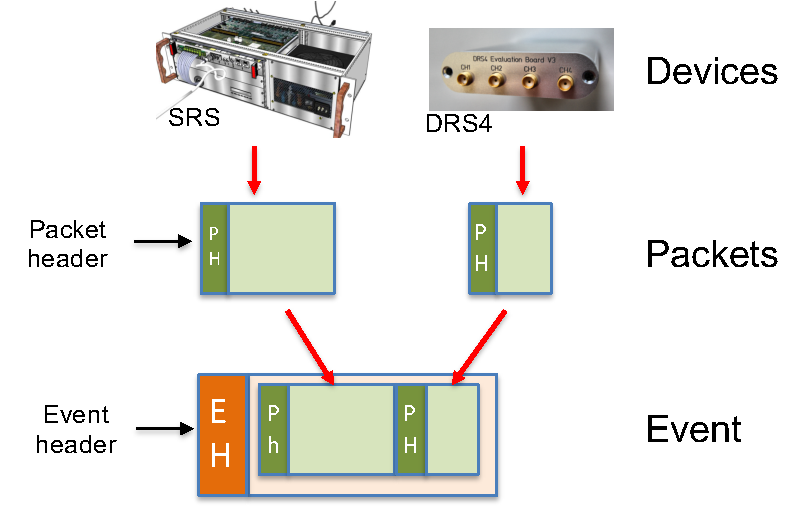
\includegraphics[width=0.9\columnwidth]{packets_events.pdf}
\end{center}
\caption{\label{packets_events} The hierarchy of data stored in a
  file. Each readout unit (in this example the SRS and the DRS4)
  generates a packet. The packets from all devices in the readlist are
  collected in an Event. Each unit can be, and usually is, of variable
  length.}
\end{figure}

This is shown in Fig.~\ref{packets_events}. Each of our two readout
devices here (the SRS and the DRS4) contribute one packet to each
Event. In this example, each Event consists of two packets.

The Packet from each device has an identifier that uniquely identifies
its origin, called the \emph{packet id}. This should be a
never-changing number (as we will see in a moment, we used packet id
1010 for the SRS, and id 1020 for the DRS4) that identifies the device
in question and, by extension, a set of readout channels of the larger
detector system that may be read out with many devices.

For example, the PHENIX electromagnetic calorimeter was read out with
about 180 ``Front-End Modules'' (FEM), each holding 144 individual
channels. Each of the Front-End Modules contributed one packet to the
Event. Such a PHENIX event had about 3200 packets from all detector
sytems combined, and the same number of unique packet ids. Since the
mapping of packet id to a particular FEM never changed, we would often
refer to a given FEM by its packet id (``we had a problem with 4072
last night'').

Each Packet has another header field, historically called the
hitformat, that identifies a decoding algorithm to unpack the data in
a way that they can be accessed through a set of standard APIs.

Different from the packet id, this hitformat has changed for several
packet types from various detectors over the lifetime of the PHENIX
experiment several times. The PHENIX Electromagnetic Calorimeter FEMs,
for example, have seen about 8 format changes, usually to achieve a
denser or faster packaging of the data in the packet payload. During
the commissioning phase of new electronics one typically adds more
information to be able to certify the correctness of the received
data, such as checksums and other debug-style information, and also
uses less sophisticated firmware for packaging the data. As one gains
confidence that everything works as specified, one applies a denser
packaging with more elaborate firmware. 

Each time the format changes for a given readout device changes, a new
hitformat identifies a new decoding algorithm that will present the
data to the user (or the analysis code) in \emph{exactly the same way}
as before, and such a change is completely transparent to the user
code. No user code will break as a result of a hitformat change.

To summarize, the packet header has two important fields:

\begin{itemize}
\item the packet id says \emph{what} is stored in the packet;
\item the hitformat says \emph{how} the payload is stored.
\end{itemize}

Although I said above that this ``Events containing Packets'' paradigm
is what one typically gets from a event/trigger-centric data
acquisition system with an event builder, our format is equally well
suited to store \emph{streaming} data, also known as a trigger-less
readout. This is what sPHENIX will use for the readout of the tracking
system, using the same format. Instead of making per-device packets
for each trigger, we \emph{packetize} the continuously streaming data
off a detector, storing them either as consecutive packets in one
event structure, or as individual packets in multiple events, or a
combination of both. Such an Event now covers a certain time range,
rather than a trigger. This is analogous to telecom Voice-Over-Ip
applications, where audio is packetized and sent through networks in a
similar way.




Using the \emph{dlist} utility that is described later in
section~\ref{tools}, we examine the aforementioned data file from 2013
with the SRS and the DRS4 packets. The \emph{dlist} utility lists the packets
that it finds in the first data event:

\begin{verbatim}
$ dlist beam_0000004094-0000.evt
Packet  1010 23262 -1 (sPHENIX Packet)  70 (IDSRSV01)
Packet  1020  5126 -1 (sPHENIX Packet)  81 (IDDRS4V1)
\end{verbatim}

You can see the two packets from the two devices (the SRS and the
DRS). The first number is the packet id, followed by the length in
Dwords (32-bit words), the packet type (-1), and the hitformat number
with a mnemonic that describes that number. The only packet type in
sPHENIX is that ``sPHENIX Packet'' denoted ``-1''; there are a number
of legacy packets that are currently still supported while we
transition to a full sPHENIX implementation.


There are a number of \emph{event types} defined, which denote a
different set of devices that are read in that event. Most types are
considered data events, and some of them are referred to as special
events. The use of different event types is easiest explained --
although they are not used at RHIC -- with the spill-on and spill-off
events. At accelerators that have a spill structure, such as the AGS,
or the CERN SPS, one would usually generate type 1 events that read
out the actual experiment. In addition, it is often necessary to
obtain information \emph{about} the most recent spill, the intensity,
effective spill length, and so on. At the begin and end of each spill
one generates spill-on and spill-off events, respectively, which read
and reset a number of scalers that count the beam signals from some
start counter during the spill, together with other relevant
information. The actual detector is not read out in those
events. \emph{Different event types read and store the data from
  different readout units.}


The most important special events are the so-called \emph{begin-run
  event}, the \emph{end-run event}, and the \emph{luminosity event} that
denotes the beginning of a new luminosity block. The begin- and
end-run events are special events that usually contain meta-data about
the data file, and so embed important information about the dataset in
the data file itself.

It is guaranteed that the begin-run event is the first event seen from
a given run, and the end-run event is the last event. In addition to
the meta data they usually contain, they serve as a convenient marker
for continuously running online monitoring processes that a new run has
begun, or that a run has ended. On receipt of a begin-run event, such
a monitoring process could, for example, clear all its monitoring
histograms, or could store all such histograms on receipt of the
end-run event.


Here are the defined event types:
     
\begin{table}[hbt]
  \caption { \label{event_types} The currently defined event types.}
\begin{center}
\begin{tabular}{|r|l|l|}
\hline
Event type & meaning & comment \\
\hline
\hline
    1 & Data Event &  Readout of detector hardware\\ \hline
    2 & Streaming Data Event &  Streaming Readout of detector hardware\\ \hline
    3 \dots 7 & Data Events & reserved for future use \\ \hline
    8  & Spill-On Event &  \\ \hline
    9  & Begin-Run Event & Automatically generated \\ \hline
    12 & End-Run Event & Automatically generated   \\ \hline
    14 & Scaler Event  &  Scaler information \\ \hline
    15 & Lumi Event  &  Denotes the start of a new Luminosity Block \\ \hline
    16 & Spill-Off Event  &  \\ \hline
\hline
\end{tabular}
\end{center}
\end{table}

The Spill-on and Spill-off events have no application in RHIC running,
but are often used during test beam data taking at accelerators with a
spill structure.

\section{Command Line Utilities}
\label{tools}

The event libraries come with a set of ready-made command line
utilities that make it easy to inspect and manipulate the event
data.

In your everyday work with sPHENIX data, you'll find that a lot can be
accomplished with these ready-made tools. Very often, someone comes up
with a new creative way to use them in combination with perl, grep, sed,
wc, and so on to get some answers about the data structure without
actually programming anything.

The most versatile tools we have are
\begin{itemize}
\item  the dlist utility, which lets you list the packets contained in a given event;

\item the ddump utility, which lets you dump and look at the contents of a packet in various ways;

\item the dpipe utility, which copies events from one destination to
  another with a lot of flexibility; you can also use this to sift
  through a data stream in a simple way.
\end{itemize}

All utilities have a -h switch to provide some online help.

Let's start with \emph{dlist}. It lists the packets it finds in the
Event, and calls the packets' identify() function on each of them, so
you'll see a short identification message for each packet found.

dlist can open any known input stream, and its default is to open a
data file. Alternatively, it can open an online monitoring stream from
the data acqusition. There is also a ``test'' stream that generates
made-up events with certain predictable properties. This test stream
lets you explore some aspects of what is described here and also in
the next chapter without the need for an actual data file.

\subsection{dlist}

We have briefly seen the output of the  \emph{dlist} utility 
before:

\begin{verbatim}
$ dlist beam_0000004094-0000.evt
Packet  1010 23262 -1 (sPHENIX Packet)  70 (IDSRSV01)
Packet  1020  5126 -1 (sPHENIX Packet)  81 (IDDRS4V1)
\end{verbatim}

dlist, ddump, and dpipe have a large number of options to modify their
behavior.  As much as possible, they are using the same event
and input selection switches.

By default,
\begin{itemize}
\item they display information from data events only -- one needs to
  explicitly ask ask for other event types. This is the most commonly
  desired behavior. Since the begin-run event is the event number 1,
  one normally sees event number 2, unless one asks for other event
  types.
\item They display only one event, and then exit.
\end{itemize}

Using the command line options, one can override the defaults in many
different ways. An important option is the
``-i'' (``identify'') option, which asks the events it selects to
print a one-line identification:

\begin{verbatim}
$ dlist -i beam_0000004094-0000.evt
 -- Event     2 Run:  4094 length: 28396 type:  1 (Data Event)  1381104934
Packet  1010 23262 -1 (sPHENIX Packet)  70 (IDSRSV01)
Packet  1020  5126 -1 (sPHENIX Packet)  81 (IDDRS4V1)
\end{verbatim}

You can see that we are listing the packets in event number 2, the
first data event.

The event selection determines the first event to display, and the
utilites show as many events as specified from that event on, obeying the
other selection criteria  (default is just 1 event).

One can select a particular event with either the ``-e $n$'' (select
event number $n$), or ``-c $n$'' (select the $n^{\rm th}$
event). These selections are \emph{not} normally equivalent; the
``-e'' asks for the event number, which is a property of the event in
question, while ``-c'' uses the position of the event in the data
file. An event retains its number property and other identifying
information when copied to a different file. If you ask for an event
number that is not found in the data file, you run through the entire
file and get no output. Still, since the combination of a run number
and the event number uniquely identifies an event, it is more common
to use the ``-e'' switch.

Here I select the event with the number 10:

\begin{verbatim}
$ dlist -i -e 10 beam_0000004094-0000.evt
 -- Event    10 Run:  4094 length: 28396 type:  1 (Data Event)  1381104934
Packet  1010 23262 -1 (sPHENIX Packet)  70 (IDSRSV01)
Packet  1020  5126 -1 (sPHENIX Packet)  81 (IDDRS4V1)
\end{verbatim}

The ``-n $n$'' switch instructs dlist to display information about $n$
events total, with the default being 1 as in the previously shown examples.

\begin{verbatim}
$ dlist -i -e 10 -n 5 /mac_home/data/srs_with_drs/beam_0000004094-0000.evt
 -- Event    10 Run:  4094 length: 28396 type:  1 (Data Event)  1381104934
Packet  1010 23262 -1 (sPHENIX Packet)  70 (IDSRSV01)
Packet  1020  5126 -1 (sPHENIX Packet)  81 (IDDRS4V1)
 -- Event    11 Run:  4094 length: 28396 type:  1 (Data Event)  1381104934
Packet  1010 23262 -1 (sPHENIX Packet)  70 (IDSRSV01)
Packet  1020  5126 -1 (sPHENIX Packet)  81 (IDDRS4V1)
 -- Event    12 Run:  4094 length: 28396 type:  1 (Data Event)  1381104934
Packet  1010 23262 -1 (sPHENIX Packet)  70 (IDSRSV01)
Packet  1020  5126 -1 (sPHENIX Packet)  81 (IDDRS4V1)
 -- Event    13 Run:  4094 length: 28396 type:  1 (Data Event)  1381104934
Packet  1010 23262 -1 (sPHENIX Packet)  70 (IDSRSV01)
Packet  1020  5126 -1 (sPHENIX Packet)  81 (IDDRS4V1)
 -- Event    14 Run:  4094 length: 28396 type:  1 (Data Event)  1381104934
Packet  1010 23262 -1 (sPHENIX Packet)  70 (IDSRSV01)
Packet  1020  5126 -1 (sPHENIX Packet)  81 (IDDRS4V1)
\end{verbatim}

Specifying ``-n 0'' means ``all events''. Be warned, though, that
certain types of streams, such as the test event stream, or an online
monitoring stream, do not have an ``end''. There are still
applications for an ``all events'' dlist (or later, ddump) with those
streams, for example, if you are looking for a particular event with
certain properties.

The ``-t'' switch selects what kind of event types are shown. ``-t''
can take the numeric event type as shown in
table~\ref{event_types}. For example, I can explicitly select the
begin-run event by

\begin{verbatim}
$ dlist -i -t 9 /mac_home/data/srs_with_drs/beam_0000004094-0000.evt
 -- Event 1 Run: 4094 length: 641 type: 9 (Begin Run Event) 1381104863
 Packet 900 491 -1 (sPHENIX Packet) 4 (IDCSTR) 
 Packet 910 142 -1 (sPHENIX Packet) 4 (IDCSTR)
\end{verbatim}

As you can see (and as described above), this event has a completely
different packet content from data events.

We can also select the end-run event type 12 (which forces dlist to go through
the entire data file):

\begin{verbatim}
$ dlist -i -t 12 beam_0000004094-0000.evt
 -- Event  3438 Run:  4094 length:     8 type: 12 (End Run Event)  1381105268
\end{verbatim}

Here we get only the event identification output, because this event
does not contain any packets in this data file. 

-t also takes ``A'' for all event types, or ``S'' for any special event type:

\begin{verbatim}
$ dlist -i -t A -n 3 beam_0000004094-0000.evt
 -- Event     1 Run:  4094 length:   641 type:  9 (Begin Run Event)  1381104863
Packet   900   491 -1 (sPHENIX Packet)   4 (IDCSTR)
Packet   910   142 -1 (sPHENIX Packet)   4 (IDCSTR)
 -- Event     2 Run:  4094 length: 28396 type:  1 (Data Event)  1381104934
Packet  1010 23262 -1 (sPHENIX Packet)  70 (IDSRSV01)
Packet  1020  5126 -1 (sPHENIX Packet)  81 (IDDRS4V1)
 -- Event     3 Run:  4094 length: 28396 type:  1 (Data Event)  1381104934
Packet  1010 23262 -1 (sPHENIX Packet)  70 (IDSRSV01)
Packet  1020  5126 -1 (sPHENIX Packet)  81 (IDDRS4V1)
\end{verbatim}

or (remember that this is an expensive command; we are reading through
the entire data file)

\begin{verbatim}
$ dlist -i -t S -n 0 beam_0000004094-0000.evt
 -- Event     1 Run:  4094 length:   641 type:  9 (Begin Run Event)  1381104863
Packet   900   491 -1 (sPHENIX Packet)   4 (IDCSTR)
Packet   910   142 -1 (sPHENIX Packet)   4 (IDCSTR)
-- Event  3438 Run:  4094 length:     8 type: 12 (End Run Event)  1381105268
\end{verbatim}

This data file does not contain any other special event types.

By the way, if you wonder what the two ``IDCSTR'' packets in the
begin-run event are, head over to the RCDAQ manual where I describe
that most setups capture RCDAQ's own setup script in packet 900. This
has become a convention, and it is quite convenient if one follows it.

Finally, there are a number of switches that determine the type of
input stream we are dealing with here. The default is a file as shown
before. One can select a ``test stream'' with the ``-T''
option, and an RCDAQ online monitoring stream with ``-r''.

The ``test stream'' allows us to explore some of the features of the
monitoring package and run through the examples without the need for
an actual data file (which might not always be easy to obtain).

\begin{verbatim}
$ dlist -T
Packet  1001    24 -1 (sPHENIX Packet)   6 (ID4EVT)
Packet  1002    36 -1 (sPHENIX Packet)   5 (ID2EVT)
Packet  1003     8 -1 (sPHENIX Packet)   6 (ID4EVT)
\end{verbatim}

The test stream only produces data events, no special events. We'll
get to the role and purpose of the 3 packets in a minute.

The ``-r'' switch connects to a running instance of RCDAQ and requests
an online event stream that is normally used for online
monitoring. Using this with dlist (or ddump) is a convenient way to
inspect events without logging data to disk, and so avoid cluttering
your storage system with data during the setup phase. The ``-r''
switch takes the hostinfo (DNS name or IP address) of the machine
running RCDAQ, and defaults to ``localhost''. Very often, the
monitoring and setup is performed on the same machine that is taking
the data. Here is RCDAQ running on a machine called ``mlpvm1'', and I
can do

\begin{verbatim}
$ dlist -i -r mlpvm1
 -- Event  5599 Run:     4 length:    16 type:  1 (Data Event)  1555272250
Packet  1003     8 -1 (sPHENIX Packet)   6 (ID4EVT)
\end{verbatim}

When I execute this on the machine itself (localhost), I can omit the name:

\begin{verbatim}
$ dlist -i -r
 -- Event  8401 Run:     4 length:    16 type:  1 (Data Event)  1555272266
Packet  1003     8 -1 (sPHENIX Packet)   6 (ID4EVT)
\end{verbatim}

``dlist -h'' lists a few more options (such as ``-I'') that are useful
if you are debugging a new packet format (a new hitformat). They are considered
expert-level switches. 


\subsection{ddump}

While dlist lists the packet in an event, \emph{ddump} displays the
contents of the packets in an interpreted and packet type-specific
way. Each packet type (that is, one for each of the about 400 defined
hitformats) has a format-specific \emph{dump()} function that
generates the output.  

All the event selection options, the ``-n'' switch, and the input
stream type specifications work exactly the same way as in dlist.

\verb|ddump -h| gives you some instructions how to use it (as does
\verb|dlist -h|). At the end of that help, there is a list of all switches:

\begin{verbatim}
  List of options:
 -e <event number>
 -c <number> get nth event (-e gives event with number n)
 -n <number> repeat for n events (0: until end of stream)
 -p <Packet Id>
 -t <event type>
 -i <print event identity>
 -I <print in-depth packet identity (default is short form)>
 -f (stream is a file)
 -T (stream is a test stream)
 -r (stream is a rcdaq monitoring stream)
 -O (stream is a legacy ONCS format file)
 -g use generic dump
 -d numbers are std::decimal (default std::hex) for generic dump
 -o numbers are octal (default std::hex) for generic dump
 -s for a generic dump, send packet raw payloadc to stdout for further manipulation
 -x like -s, but also include the packet header
 -v verbose
 -h this message
\end{verbatim}

We'll go through a few of them now.


The output from our example data file from 2013 is large, we'll
start with a test stream:

\begin{verbatim}
 $ ddump -T
Packet  1001    24 -1 (sPHENIX Packet)   6 (ID4EVT)
    0 |  00000000 00000001 00000002 00000003
    4 |  00000004 00000005 00000006 00000007
    8 |  00000008 00000009 0000000a 0000000b
   12 |  0000000c 0000000d 0000000e 0000000f
   16 |  00000010 00000011 00000012 00000013

Packet  1002    36 -1 (sPHENIX Packet)   5 (ID2EVT)
    0 |  0000 0001 0002 0003 0004 0005 0006 0007
    8 |  0008 0009 000a 000b 000c 000d 000e 000f
   16 |  0010 0011 0012 0013 0014 0015 0016 0017
   24 |  0018 0019 001a 001b 001c 001d 001e 001f
   32 |  0020 0021 0022 0023 0024 0025 0026 0027
   40 |  0028 0029 002a 002b 002c 002d 002e 002f
   48 |  0030 0031 0032 0033 0034 0035 0036 0037
   56 |  0038 0039 003a 003b 003c 003d 003e 003f

Packet  1003     8 -1 (sPHENIX Packet)   6 (ID4EVT)
    0 |  fffffff4 fffffff9 fffffcaa 00003a5f

\end{verbatim}

So we see human-readable presentations of the 3 packets in that
made-up event. The first packet pretends to be an ADC with 20
channels, where channel $i$ always holds the value $i$ ( 0..19).
Likewise, packet 1002 holds the value $i$ in channel $i$ for 64
channels. This packet internally holds 16-bit values, rather than
32-bit values for packet 1001. This makes the test data suitable for
testing different aspects of the data handling, sich as the proper
byte swapping, transfers, and a number of other things.

The test data have in the past been used to make simple checks of the
proper working of the analysis code, because the mean of the signals
of a given channel must be the channel number when one uses packet
1001 or 1002.

Packet 1003 holds 4 32-bit values, which are 4 different random
numbers of different scales with a gaussian distribution with mean = 0
and a RMS = 10,100,1000, and 10000 for the 4 ``channels''.

While these are pseudo-random numbers, they always start with the same
seed value and give a predictable sequence of numbers, which is
suitable for most ``training'' applications we have in mind
here. These are not high-quality random sequences and should not be
used for applications that require those.

Usually, our events have a large number of packets. You typically want
to select a particular packet, or a small number of them. That is
accomplished with the ``-p'' option. You can specify a single packet
number, a comma-separated list of packets, a range specifier with a
minus sign, or any combination thereof. These are examples of valid
packet id selections:

\begin{verbatim}
ddump  -p 1003
ddump  -p 1003,2000,2006
ddump  -p 1001,1003,2000-2006
ddump  -p 1001,1002,1003,2000-2006,3005-4000,5001,5002,6000-6005
\end{verbatim}
The selection must not contain spaces. 

We will be using the ``-p 1003'' option to see the random numbers in
packet 1003 for a number of events:

\begin{verbatim}
$ ddump -T -p 1003 -n 10
Packet  1003     8 -1 (sPHENIX Packet)   6 (ID4EVT)
    0 |  fffffff4 fffffff9 fffffcaa 00003a5f

Packet  1003     8 -1 (sPHENIX Packet)   6 (ID4EVT)
    0 |  00000007 ffffffd6 ffffff05 ffffdcd4

Packet  1003     8 -1 (sPHENIX Packet)   6 (ID4EVT)
    0 |  00000006 00000018 00000157 ffffb5a3

Packet  1003     8 -1 (sPHENIX Packet)   6 (ID4EVT)
    0 |  0000000e ffffffdb 000003d6 ffffef1a

Packet  1003     8 -1 (sPHENIX Packet)   6 (ID4EVT)
    0 |  0000000c ffffff84 000003fa 0000192e

Packet  1003     8 -1 (sPHENIX Packet)   6 (ID4EVT)
    0 |  00000008 00000031 fffffd5e ffffc1cc

Packet  1003     8 -1 (sPHENIX Packet)   6 (ID4EVT)
    0 |  ffffffff 000000a0 00000006 00004a8d

Packet  1003     8 -1 (sPHENIX Packet)   6 (ID4EVT)
    0 |  00000004 00000067 fffff887 fffffc89

Packet  1003     8 -1 (sPHENIX Packet)   6 (ID4EVT)
    0 |  fffffffe ffffff08 0000066f 00001dd9

Packet  1003     8 -1 (sPHENIX Packet)   6 (ID4EVT)
    0 |  fffffff8 ffffffae ffffff48 000046bb
\end{verbatim}

where each event delivers different numbers in that packet.


There are different ways of displaying the data. By default, one gets
the standard, interpreted, and as much as possible human-readable
presentation of the data, which in the case of the ``ID2EVT'' and
``ID4EVT'' hitformats in the test events happens to be a simple
hexadecimal listing. I will show you better examples of the usefulness
of these tailored, format-specific presentations in a minute.

ddump can also provide a simple hex-dump of the data, called a
``generic'' dump, and can also make a generic dump in decimal
format. The generic format is requested with the ``-g'' option, which
defaults to hexadecimal, and ``-d'' requests a decimal generic dump.

We can see this here, where we display the same random number
sequences in decimal:

\begin{verbatim}
$ ddump -T -p 1003 -g -d -n 10
Packet  1003     8 -1 (sPHENIX Packet)   6 (ID4EVT)
    0 |         -12         -7       -854      14943

Packet  1003     8 -1 (sPHENIX Packet)   6 (ID4EVT)
    0 |           7        -42       -251      -9004

Packet  1003     8 -1 (sPHENIX Packet)   6 (ID4EVT)
    0 |           6         24        343     -19037

Packet  1003     8 -1 (sPHENIX Packet)   6 (ID4EVT)
    0 |          14        -37        982      -4326

Packet  1003     8 -1 (sPHENIX Packet)   6 (ID4EVT)
    0 |          12       -124       1018       6446

Packet  1003     8 -1 (sPHENIX Packet)   6 (ID4EVT)
    0 |           8         49       -674     -15924

Packet  1003     8 -1 (sPHENIX Packet)   6 (ID4EVT)
    0 |          -1        160          6      19085

Packet  1003     8 -1 (sPHENIX Packet)   6 (ID4EVT)
    0 |           4        103      -1913       -887

Packet  1003     8 -1 (sPHENIX Packet)   6 (ID4EVT)
    0 |          -2       -248       1647       7641

Packet  1003     8 -1 (sPHENIX Packet)   6 (ID4EVT)
    0 |          -8        -82       -184      18107

\end{verbatim}



Let's go back to the file taken in 2013 with the DRS4 and the SRS data:
\begin{verbatim}
$ dlist -i beam_0000004094-0000.evt
 -- Event     2 Run:  4094 length: 28396 type:  1 (Data Event)  1381104934
Packet  1010 23262 -1 (sPHENIX Packet)  70 (IDSRSV01)
Packet  1020  5126 -1 (sPHENIX Packet)  81 (IDDRS4V1)
\end{verbatim}

and ddump the DRS4 packet. The chosen presentation of the data
is one line per sample (1024 in this case), with columns for the
sample number, the time, and then the sample values of the 4 inputs.



I have cut out a number of lines and show the beginning and the end of
the long output, and in the middle a section where one can actually see a
negative-going pulse in the data of channel 1, around sample  292:

\begin{verbatim}
$ ddump -p 1020 beam_0000004094-0000.evt
Packet  1020  5126 -1 (sPHENIX Packet)  81 (IDDRS4V1)
 Samples 1024  enabled channnels:   0  1  2  3
   ch |       time          ch0          ch1          ch2          ch3
    0 |          0         -2.2         -1.4         -1.3         -0.4
    1 |   0.992839         -0.8         -2.5         -1.8         -1.7
    2 |    1.98568         -2.6         -2.5           -1         -0.1
    3 |    2.97852         -1.8         -1.5         -3.5         -3.2
    4 |    3.97135           -2         -1.2         -1.2         -1.1
    5 |    4.96419         -2.9         -2.1         -3.6         -3.3
    6 |    5.95703           -1          0.3         -1.4         -1.1
    7 |    6.94987         -2.9         -2.9         -3.7         -2.4
    8 |    7.94271         -1.8           -2         -1.5         -0.9
    9 |    8.93555         -1.8         -2.8         -3.6         -2.5
   10 |    9.92839         -2.8         -2.7           -3         -2.4
   11 |    10.9212         -3.1         -4.1         -3.7         -4.2
   12 |    11.9141         -2.9         -2.9         -0.7         -0.9
   13 |    12.9069           -4         -3.9         -2.7         -3.5
   14 |    13.8997         -3.5         -2.8         -2.6         -1.9

   ...

  287 |    284.945         -0.6         -0.6        -43.8        -66.8
  288 |    285.938         -2.1         -2.1        -40.6        -58.7
  289 |     286.93         -0.4         -1.4        -37.2        -54.3
  290 |    287.923         -1.6         -1.4          -30        -47.5
  291 |    288.916         -0.2         -4.9        -28.6        -43.8
  292 |    289.909         -2.1        -17.4        -24.4        -34.9
  293 |    290.902            0        -38.5        -24.6        -31.2
  294 |    291.895           -1        -85.5        -21.1        -26.1
  295 |    292.887          0.1       -189.8        -20.2        -25.3
  296 |     293.88         -1.5       -272.6          -18        -23.3
  297 |    294.873            0       -392.6        -18.3        -19.3
  298 |    295.866           -4       -402.5          -16          -18
  299 |    296.859         -3.7       -378.3        -15.4        -19.5
  300 |    297.852         -4.5       -318.7        -14.9        -13.2
  301 |    298.844         -3.6       -271.8        -14.4        -12.4
  302 |    299.837         -3.1       -204.3        -10.9         -9.8
  303 |     300.83         -1.1       -154.7        -12.6           -9
  304 |    301.823         -2.1       -134.8         -9.5         -7.9
  305 |    302.816            1       -103.3        -10.8         -8.5
  306 |    303.809          0.7        -84.2         -7.9         -6.6
  307 |    304.801          1.5        -70.1         -8.7         -6.7
  308 |    305.794          1.2        -59.6         -7.2         -3.6
  309 |    306.787          0.6        -56.4         -7.9         -7.2
  310 |     307.78          0.1        -52.3         -7.1         -3.3
  311 |    308.773         -0.4        -52.3         -9.2           -7
  312 |    309.766         -2.1          -52         -7.8         -6.3
  313 |    310.758         -1.8        -47.4         -9.6         -9.6
  314 |    311.751         -3.6        -46.3         -8.8         -6.3
  315 |    312.744         -3.5        -42.6        -10.6         -8.7
  316 |    313.737         -6.1        -38.8         -9.5         -7.4

  ...

 1018 |    1010.71         -2.9           -2         -2.4         -3.1
 1019 |     1011.7         -5.2         -3.7         -6.8         -7.5
 1020 |     1012.7         -5.1         -2.8           -3         -2.6
 1021 |    1013.69         -4.4         -3.5         -3.6         -3.7
 1022 |    1014.68         -4.9         -1.8         -2.5         -1.9
 1023 |    1015.67         -2.8         -2.1         -3.1         -2.8
\end{verbatim}


Fig.~\ref{drs4_waveform} shows that same waveform as a plot.


\begin{figure}[htb]
\begin{center}
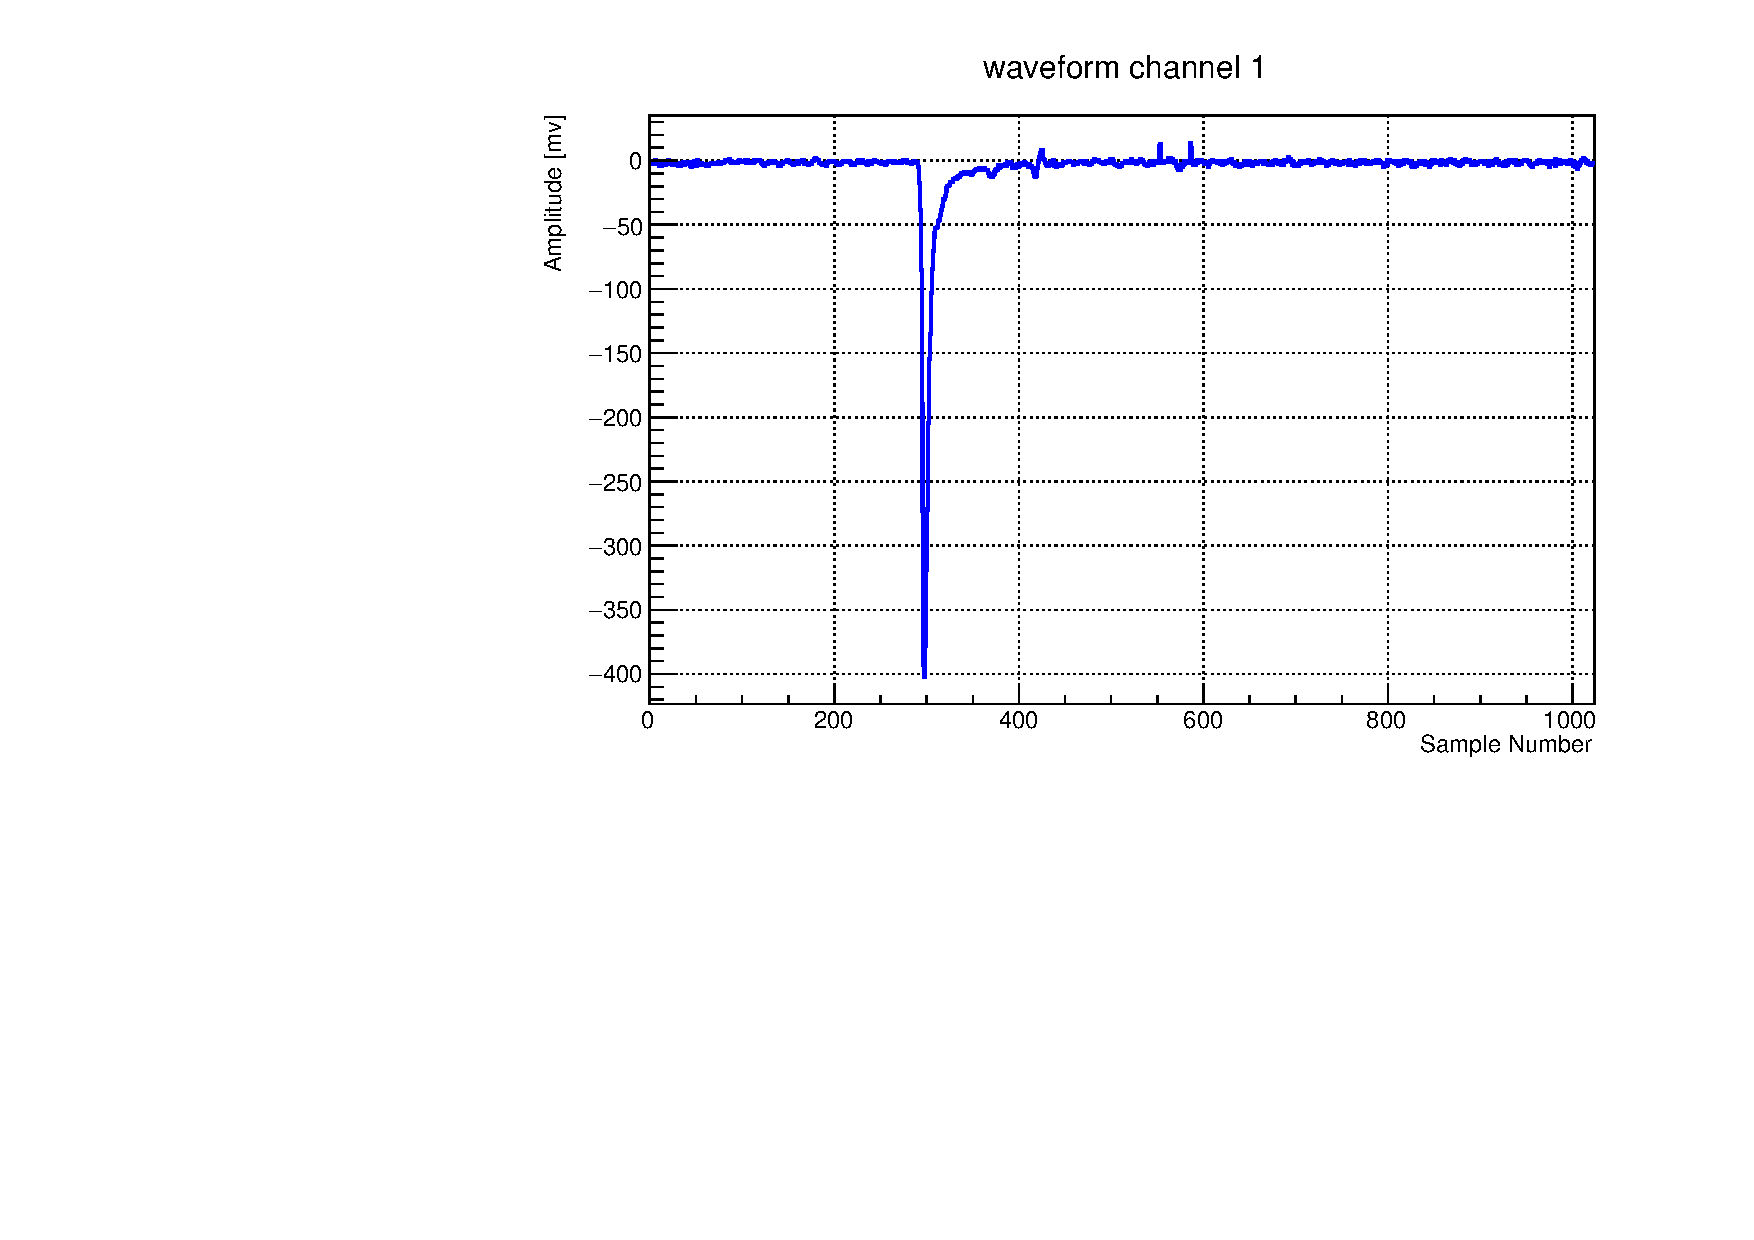
\includegraphics[width=0.9\columnwidth]{drs4_waveform.pdf}
\end{center}
\caption{\label{drs4_waveform}The plot of the waveform of channel 1
  shown in the DRS4 ddump output.
}
\end{figure}



\begin{figure}[htb]
\begin{center}
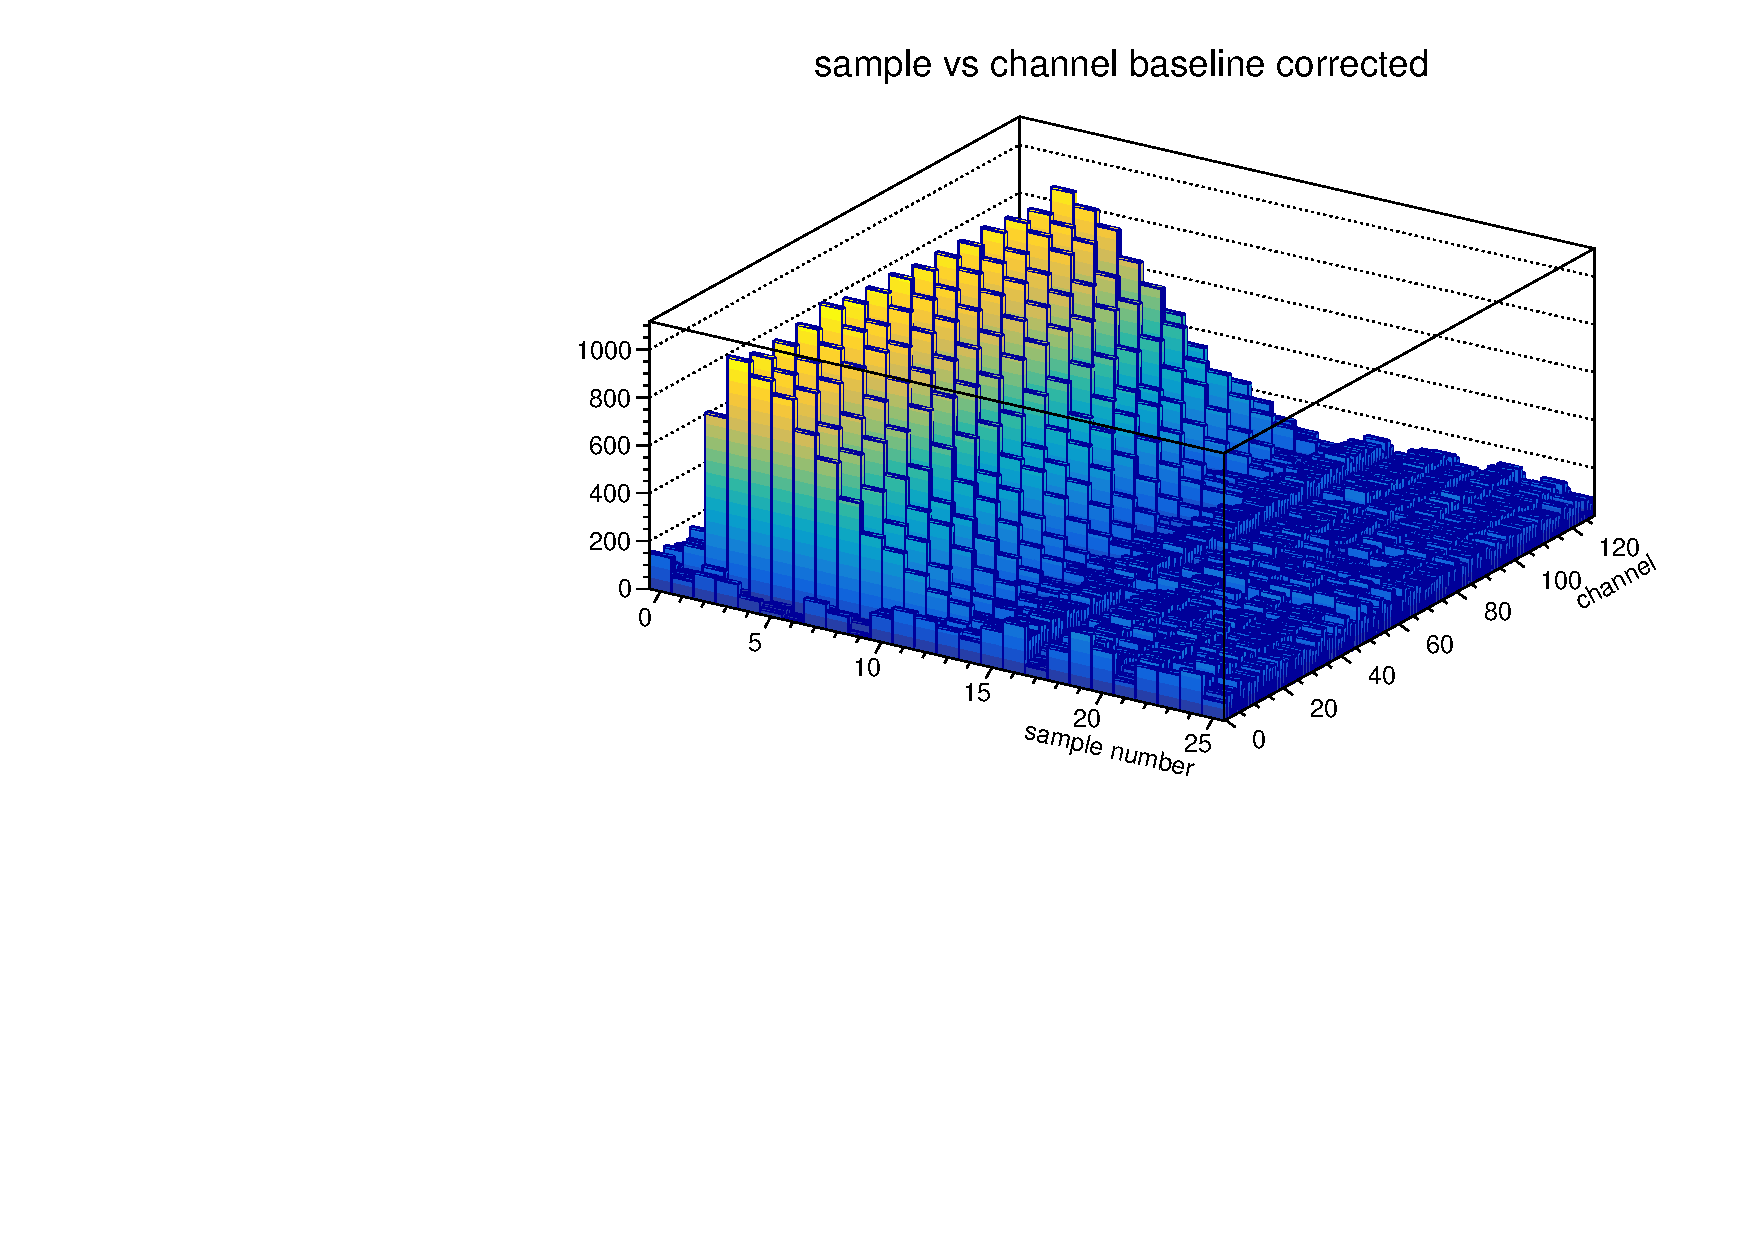
\includegraphics[width=0.9\columnwidth]{srs_display.pdf}
\end{center}
\caption{\label{srs_display} This is the visualization of the SRS dump
  shown in the text. The plot shows the channel numbers vs
  sample number, with the z axis showing the pulse height. This plot
  applies a baseline correction and also inverts the ADC values, so
  the negative-going pulses show up as positive values.  }
\end{figure}



The SRS data in the same event file have a completely different
format, and ddump presents the data in a very different way suitable
for the composition of the data. The SRS system has up to 16 so-called
\emph{APV25 Hybrids} with 128 individual channels each, and each
channel can sample a waveform with up to 28 samples (the DRS4 can
sample up to 1024 samples, as shown above).

The SRS-specific dump function displays each waveform across the
screen, and one line per channel, one block of such 128-channel data
for each hybrid. I am showing here a dump from a different data file,
one where I set the Hybrids up in ``test pulse mode'', where they
auto-generate known test pulses on a number of channels. This can be
used to test the proper functioning of the Hybrids. The test pulses
can be seen in figure~\ref{srs_display}, which shows the channel
numbers vs sample number, with the z axis showing the pulse
height. 



In this case, we selected the maximum of 28 samples, and the SRS
system had 4 hybrids connected.

I only show part of one block of the output; the entire output consists of 4 such blocks:

%{\fontsize{4.5}{3}\selectfont\obeyspaces\obeylines
%\tt
\begin{Verbatim}[fontsize=\tiny]
ddump -p 1020 srs-00000001-0000.evt
Packet  1020  8122 -1 (sPHENIX Packet)  70 (IDSRSV01)
Number of Hybrids: 4

Framecounter: 0
HDMI Channel: 0
Description:  ADC
Words:        4050
Time samples: 28
Sample     0    1    2    3    4    5    6    7    8    9   10   11   12   13   14   15   16   17   18   19   20   21   22   23   24   25   26   27
Addr     156  159  153  152  128  129  135  132  128  131  129  128  224  225  227  224  228  231  225  224  248  249  255  252  240  243  241  240
Error      0    0    0    0    0    0    0    0    0    0    0    0    0    0    0    0    0    0    0    0    0    0    0    0    0    0    0    0
       ----------------------------------------------------------------------------------------
   0 |  3060 3049 3206 3155 3094 3103 3216 3169 3148 3146 3203 3050 3026 3011 3091 3163 3106 3026 3168 3096 2983 3035 3165 3030 3064 3059 3160 3056
   1 |  3019 2993 3160 3165 3108 3057 3174 3148 3091 3046 3125 3042 3059 2979 3039 3152 3064 2965 3104 3095 2985 2993 3108 3041 3058 2995 3101 3070
   2 |  3011 2980 3142 3156 3091 3052 3175 3163 3111 3064 3133 3060 3075 2967 3028 3140 3075 2973 3135 3088 2970 2985 3094 3035 3057 2995 3086 3057
   3 |  3009 2965 3113 3146 3093 3045 3171 3149 3081 3034 3117 3029 3023 2956 3004 3102 3030 2959 3119 3100 2963 2960 3063 3008 3030 2979 3070 3037
   4 |  3012 2802 2365 2097 2073 2157 2360 2456 2540 2613 2769 2761 2821 2797 2879 2995 2960 2902 3069 3076 2978 2981 3083 3033 3058 2984 3070 3051
   5 |  3007 2969 3113 3176 3116 3076 3195 3181 3122 3060 3126 3048 3056 2986 3042 3147 3036 2953 3105 3114 2990 3004 3102 3047 3070 2997 3087 3057
   6 |  2989 2942 3119 3147 3074 3038 3169 3135 3087 3034 3123 3022 3014 2955 3008 3093 3033 2940 3099 3076 2965 2978 3100 3037 3042 2979 3071 3025
   7 |  3016 2977 3149 3175 3095 3048 3176 3147 3066 3017 3098 3013 3039 2974 3021 3128 3052 2966 3096 3084 2976 3001 3094 3025 3061 2999 3069 3030
   8 |  3032 2990 3154 3175 3126 3073 3176 3169 3113 3063 3158 3086 3086 3000 3054 3159 3085 2983 3125 3122 3005 3014 3121 3041 3040 2994 3087 3065
   9 |  2997 2976 3132 3168 3065 3024 3160 3135 3087 3048 3111 3018 3042 2951 3006 3105 3024 2950 3099 3073 2959 2969 3065 3019 3047 2985 3058 3047
  10 |  3001 2955 3120 3157 3073 3045 3175 3154 3092 3030 3111 3017 3016 2950 3021 3128 3038 2946 3112 3102 2995 3001 3088 3011 3039 2984 3062 3017
  11 |  2992 2942 3104 3168 3088 3029 3169 3152 3080 3044 3121 3037 3050 2971 3015 3124 3041 2945 3084 3071 2960 2971 3077 3018 3035 2973 3068 3050
  12 |  2967 2751 2347 2095 2070 2147 2367 2451 2524 2589 2743 2735 2804 2792 2872 2999 2973 2897 3057 3056 2945 2961 3059 3005 3026 2968 3040 3022
  13 |  2995 2944 3077 3150 3079 3070 3175 3155 3086 3046 3120 3039 3055 2970 3009 3114 3038 2958 3096 3095 2991 2994 3090 3026 3070 2996 3070 3049
  14 |  3018 2973 3125 3130 3036 3007 3165 3146 3086 3016 3076 2991 2999 2939 3002 3096 3039 2953 3100 3063 2941 2948 3077 3022 3043 2986 3060 3037
  15 |  3004 2964 3116 3167 3075 3032 3164 3138 3072 3037 3115 3023 3037 2963 3006 3101 3031 2943 3086 3107 2987 2987 3058 3005 3035 2971 3050 3041
  16 |  3014 2986 3151 3166 3094 3043 3168 3141 3066 3027 3111 3050 3058 2969 3019 3140 3072 2980 3127 3109 2991 2998 3094 3046 3063 2994 3082 3056
  17 |  2991 2966 3127 3167 3072 3017 3139 3093 3052 3024 3108 3007 3011 2935 2978 3089 3015 2941 3075 3075 2963 2970 3049 2991 3029 2969 3050 3028
  18 |  2987 2957 3118 3151 3056 3020 3148 3118 3054 2995 3078 3003 3018 2948 2999 3091 3017 2933 3073 3060 2950 2961 3060 2979 2996 2942 3029 3018
  19 |  3005 2969 3135 3168 3093 3045 3160 3131 3063 3031 3109 3027 3038 2970 3008 3089 3014 2935 3077 3082 2979 2986 3071 3008 3030 2976 3058 3040
  20 |  2996 2781 2355 2114 2086 2147 2359 2450 2532 2603 2751 2759 2826 2797 2875 3001 2950 2896 3056 3059 2959 2974 3069 2999 3041 3005 3090 3068
  21 |  3020 2977 3115 3161 3092 3056 3170 3149 3089 3060 3123 3040 3045 2964 3013 3109 3033 2949 3089 3098 2979 2986 3081 3018 3046 2993 3083 3061
  22 |  2976 2943 3107 3132 3055 3024 3161 3118 3074 3020 3087 3018 2996 2939 3003 3121 3052 2949 3068 3059 2944 2943 3043 3000 3025 2971 3045 3028
...

 124 |  2960 2876 2875 2813 2821 2798 2921 2970 2922 2903 2975 2911 2931 2892 2953 3048 2963 2892 3056 3042 2944 2958 3048 2982 2995 2935 3013 2998
 125 |  2965 2920 3053 3068 2986 2958 3102 3067 3005 2984 3075 2980 2985 2915 2960 3042 2969 2903 3044 3034 2939 2939 3017 2968 2986 2933 3012 2992
 126 |  2977 2953 3093 3103 3017 2987 3106 3091 3041 3008 3086 2996 3006 2927 2976 3077 3017 2943 3089 3078 2966 2968 3057 2990 3034 2975 3047 3020
 127 |  2781 2789 2802 2807 2766 2786 2801 2805 2852 2871 2864 2815 2831 2776 2767 2787 2817 2819 2881 2870 2862 2812 2833 2799 2828 2802 2827 2854
\end{Verbatim}

One can see the test pulses in the numbers starting around sample 2 in channels 4, 12, 20, and so on.


Let me mention two more switches to \verb|ddump|, \verb|-s| and
\verb|-x|. Rather than doing anything with the packet's data, these
switches make ddump put the raw data out to stdout, and you can pipe
the into any utility to work with the data, such as \verb|od|. The
aforementioned hexadecimal, decimal, or octal dumps are just a tiny
subset of what, for example, \verb|od| can do, and rather than
re-inventing the functionality, this allows us to work with the data
in a myriad of ways. The difference between \verb|-s| and \verb|-x| is
that the latter also includes the packet header, not just the packet's
payload as \verb|-s| does.

Let me show one example of where this was really useful. Here is a file
where we read out our DREAM electronics at Fermilab, and let's say
that we are debugging the decoding (not that you as the end user would
need to do that). The generic dump shows

\begin{verbatim}
$ ddump -g dream-00002190-0000.evt | more
Packet  3000 19174 -1 (sPHENIX Packet) 103 (IDDREAMV0)
    0 |  ccddaabb 5e176400 64600000 8b610160
    4 |  483403e0 97b260b9 76816830 64815001
    8 |  5b815a01 5b817a81 5f015181 52816301
   12 |  57815781 4f815881 71016481 49816881
   16 |  64815001 69016b81 4a817681 93015001
   20 |  64813f01 6b815481 39015181 60014701
   24 |  64815501 66015b81 5a015901 54814381
   28 |  34815881 43815281 50014981 5d815601
   32 |  51815601 4b016301 3d816301 4c813f01
   ....
\end{verbatim}

There are two problems. First, the DREAM data are inherently 16bit
values, and the firmware formats them internally in big-endian
byte-ordering. At a glance, when one compares the data with the format
descritption, it is not always easy to identify the DREAM-internal
markers that denote the different fields. Here is a better view of the
raw data as hex dump that lets you see the field values in their
``natural'' representation:

\begin{verbatim}
$ ddump -s -g dream-00002190-0000.evt | od -t x2 --endian=big | more
0000000 bbaa ddcc 0064 175e 0000 6064 6001 618b
0000020 e003 3448 b960 b297 3068 8176 0150 8164
0000040 015a 815b 817a 815b 8151 015f 0163 8152
0000060 8157 8157 8158 814f 8164 0171 8168 8149
0000100 0150 8164 816b 0169 8176 814a 0150 0193
0000120 013f 8164 8154 816b 8151 0139 0147 0160
0000140 0155 8164 815b 0166 0159 015a 8143 8154
0000160 8158 8134 8152 8143 8149 0150 0156 815d
0000200 0156 8151 0163 014b 0163 813d 013f 814c
0000220 0144 814a 8162 8126 813d d158 5150 5c80
0000240 5e09 d92e c1fc 3453 398c b2b9 b268 0114
0000260 0127 811a 012d 0122 8152 8108 0142 8120
0000300 8145 0112 815b 8065 8000 8000 0127 012d   ....
\end{verbatim}

Of course, the DREAM format has its dedicated way of displaying the
information for easy reading:

\begin{Verbatim}[fontsize=\tiny]

$ ddump  /mac_home/data/dream/dream-00002190-0000.evt | more
Packet  3000 19174 -1 (sPHENIX Packet) 103 (IDDREAMV0)
Nr of FEUs:            1
FEU_ID:                 0 100
 DreamChips:            8  enabled:   1  1  1  1  1  1  1  1
 Nr of samples:        64
 Pedestal subtracted    0
 Zero suppressed        0
 Common Noise supp.     0
                                      ---- Dream chip 0 ----
 ch->     0    1    2    3    4    5    6    7    8    9   10   11   12   13   14   15   16   17   18   19   20   21   22   23   24   25   26   27   28   29   30   31
smple|   32   33   34   35   36   37   38   39   40   41   42   43   44   45   46   47   48   49   50   51   52   53   54   55   56   57   58   59   60   61   62   63
-----+-----+----+----+----+----+----+----+----+----+----+----+----+----+----+----+----+----+----+----+----+----+----+----+----+----+----+----+----+----+----+----+----+
   0 |  374  336  356  346  347  378  347  337  351  355  338  343  343  344  335  356  369  360  329  336  356  363  361  374  330  336  403  319  356  340  363  337
    -   313  327  352  341  356  347  358  345  346  323  340  344  308  338  323  329  336  342  349  342  337  355  331  355  317  319  332  324  330  354  294  317
   1 |  366  332  346  344  346  376  344  334  348  350  341  344  342  346  331  360  367  359  328  334  350  366  359  373  332  327  398  313  353  340  363  338
    -   318  326  350  340  360  347  360  341  346  333  341  337  306  336  321  329  335  348  347  345  338  353  332  357  320  320  331  321  323  351  302  317
   2 |  366  338  338  341  349  376  347  330  348  355  344  346  342  345  329  353  368  361  330  333  356  368  356  374  326  328  398  313  356  342  364  338
    -   325  332  349  344  361  352  358  346  345  334  343  337  308  339  322  337  330  351  344  347  346  353  336  363  320  332  341  329  326  355  309  320
   3 |  357  340  333  339  351  374  348  327  352  347  339  338  337  348  336  343  364  365  332  327  352  363  351  373  331  327  395  321  357  334  363  330
    -   318  329  355  344  360  351  356  346  343  327  342  336  304  334  323  334  328  349  343  346  350  349  342  361  313  328  333  330  325  355  312  319
   4 |  348  340  336  338  354  370  357  328  356  339  340  334  339  344  338  340  363  364  335  335  351  359  348  371  323  331  395  325  356  332  368  334
    -   319  326  350  342  356  354  358  342  345  323  342  333  297  331  327  336  327  343  352  337  350  344  340  354  313  322  334  328  319  357  306  316
  ...
\end{Verbatim}



Especially the \emph{ddump} command has in the past proven very
versatile to quickly inspect the data packets. Simple-minded analyses
have been performed just with a combination of ddump, and other
parsing utilities such as grep, awk, sed, and the like.




\section{\pmonitor}

\pmonitor\ is an online monitoring and analysis package that builds on
top of the Event Libraries for online monitoring and data analysis in
the ROOT environment. \pmonitor\ is often used as the
monitoring/analysis framework for data taken with the RCDAQ data
acquisition system. 

What does one want in an online monitoring system? Let's first say
what we do \emph{not} want: A system where you analyze a number of
events, for, say, 20 minutes, and only then get to see your
results. That clearly does not qualify as online monitoring.

Rather, one would want a system where at any time one can display,
clear, fit, and in general interact with histograms \emph{while} they
are being filled.

That does not prevent the user from setting up more static
``billboard-style'' displays that cycle through a number of displays,
but one still wants that interactivity to be able to drill down on
problems if they become apparent.

\pointout{If one leaves the online monitoring features alone,
  \pmonitor\  serves as a feature-rich off\/line analysis package. The
  online monitoring process can, without modifications, replay files,
  and form the basis for the eventual off\/line, batch-style analysis.
}

\subsection{Getting started}

Very often, you inherit an already existing \pmonitor\ project from
someone, and adjust it to your needs. Such projects are meant to be
\emph{simple} and straightforward, so if you inherit a huge project
with lots of apparent dead code, consider starting over.

In order to get a fresh, empty project, get yourself a new, empty
directory, pick a name for your project, say, ``MyTest'', and run
\verb|writePmonProject.sh|:

\begin{verbatim}
$ mkdir MyTest
$ cd MyTest
$ writePmonProject.sh MyTest
creating project MyTest
$
\end{verbatim}

(The older \verb|writePmonProject.pl| still works and creates the same
project, but it is deprecated.)

The directory name and project name are completely independent. You
should always choose a fresh, empty directory unless you know exactly
what you are doing. It is just easier this way.

At this point, you have a skeleton \pmonitor\ project that doesn't do
anything useful yet, of course. The above command gets you

\begin{verbatim}
$ ls -l
total 24
lrwxrwxrwx 1 purschke sphenix  15 Sep 26 16:42 Makefile -> MyTest.Makefile
-rw-r--r-- 1 purschke sphenix 154 Sep 26 16:42 MyTest.C
-rw-r--r-- 1 purschke sphenix 610 Sep 26 16:42 MyTest.cc
-rw-r--r-- 1 purschke sphenix 196 Sep 26 16:42 MyTest.h
-rw-r--r-- 1 purschke sphenix  80 Sep 26 16:42 MyTestLinkDef.h
-rw-r--r-- 1 purschke sphenix 852 Sep 26 16:42 MyTest.Makefile
-rw-r--r-- 1 purschke sphenix 140 Sep 26 16:42 MyTest.sh
$
\end{verbatim}

Besides the source files, you also get \verb|MyTest.C|, a small ROOT
macro that loads the library and opens a data file with
\verb|pfileopen()|, and \verb|MyTest.sh|, which starts root with that
macro, so that \verb|bash MyTest.sh myfile.evt| gets you a running
\pmonitor\ session in one step. Below we go through these steps by
hand first, so you see what is happening.

While the project doesn't do anything useful yet, it already
compiles. We will go through the mechanics of \pmonitor\ with this
empty skeleton project for a moment.

Run ``make''. It will compile everything and you will end up with a
shared library \verb|libMyTest.so| that you can load in root.

\begin{verbatim}
$ ls -l
total 68
-rwxr-xr-x 1 purschke sphenix 32960 Sep 26 16:42 libMyTest.so
lrwxrwxrwx 1 purschke sphenix    15 Sep 26 16:42 Makefile -> MyTest.Makefile
-rw-r--r-- 1 purschke sphenix   154 Sep 26 16:42 MyTest.C
-rw-r--r-- 1 purschke sphenix   610 Sep 26 16:42 MyTest.cc
-rw-r--r-- 1 purschke sphenix  2974 Sep 26 16:42 MyTest_dict.C
-rw-r--r-- 1 purschke sphenix   849 Sep 26 16:42 MyTest_dict_rdict.pcm
-rw-r--r-- 1 purschke sphenix   196 Sep 26 16:42 MyTest.h
-rw-r--r-- 1 purschke sphenix    80 Sep 26 16:42 MyTestLinkDef.h
-rw-r--r-- 1 purschke sphenix   852 Sep 26 16:42 MyTest.Makefile
-rw-r--r-- 1 purschke sphenix   140 Sep 26 16:42 MyTest.sh
$
\end{verbatim}

At this point, the next actions differ a bit depending on whether you
are using ROOT version 5 or 6. I recommend to use version~6, since a
few \pmonitor\ features are only available in that version. We stick
with the sequence for ROOT~6 for now.

For ROOT~6, you need to define an include path to tell ROOT where to
look for include files. Execute (or, to make it persistent, add it to your
\$HOME/.bash\_login or other login file):

\begin{verbatim}
export ROOT_INCLUDE_PATH=$ONLINE_MAIN/include:$ONLINE_MAIN/include/Event:$ONLINE_MAIN/include/pmonitor
\end{verbatim}

\subsection{Running \pmonitor}

Then fire up root, and try the following:
\begin{verbatim}
$ root -l
root [0] #include "MyTest.h"
root [1] .L libMyTest.so
Welcome to pmonitor.  Type phelp() for help
\end{verbatim}

Although this projects is just an empty skeleton, we can still use it
to ``monitor'' a few events, although we don't actually do anthing with them yet.

We use the \verb|testEventiterator| that I described before. In
\pmonitor, one opens one with the command \verb|ptestopen()|. We
then use the \verb|pstatus()| command to see what's going on:

\begin{verbatim}
root [2] ptestopen();
root [3] pstatus();
Not running  Stream open:   -- testEventiterator (standard)
\end{verbatim}

So we see that we have a \verb|testEventiterator| open, but we have
not started any processing of data yet (``Not running''). In order to
start processing a batch of 1000 events, we use

\begin{verbatim}
root [4] prun(1000);
\end{verbatim}

Since there is no actual analysis going on, the \verb|prun| command
will complete almost instantaneously. How can we see that we are
actually processing events? We use the \verb|pidentify(3)| command to
request that the next 3 events print out their ``identify''
information. After that, after we issue the next \verb|prun(1000)|
command for the next batch of 1000 events, we see 3 lines, identifying events
1001...1003:

\begin{verbatim}
root [5] pidentify(3); 
root [6] prun(1000); 
 -- Event 1001 Run: 1331 length: 76 type: 1 (Data Event) 1558100410 
 -- Event 1002 Run: 1331 length: 76 type: 1 (Data Event) 1558100410
 -- Event 1003 Run: 1331 length: 76 type: 1 (Data Event) 1558100410
\end{verbatim}

We are processing 1000 events, but we have requested only 3 events to
identify themselves; the next 997 events go by silently. But it shows
that with the first \verb|prun(1000)| command we did indeed process
1000 events.

We then repeat the sequence and see that we are now processing events
2000 through 2003 -- again the remaining events go by silently.

\begin{verbatim}
root [7] pidentify(3);
root [8] prun(1000);
 -- Event  2001 Run:  1331 length:    76 type:  1 (Data Event)  1558100414
 -- Event  2002 Run:  1331 length:    76 type:  1 (Data Event)  1558100414
 -- Event  2003 Run:  1331 length:    76 type:  1 (Data Event)  1558100414
root [9] .q
\end{verbatim}

We end this root session at this point. Here is the entire session again:

\begin{verbatim}
$ root -l
root [0] #include "MyTest.h"
root [1] .L libMyTest.so
Welcome to pmonitor.  Type phelp() for help
root [2] ptestopen();
root [3] pstatus();
Not running  Stream open:   -- testEventiterator (standard)
root [4] prun(1000);
root [5] pidentify(3);
root [6] prun(1000);
 -- Event  1001 Run:  1331 length:    76 type:  1 (Data Event)  1558100410
 -- Event  1002 Run:  1331 length:    76 type:  1 (Data Event)  1558100410
 -- Event  1003 Run:  1331 length:    76 type:  1 (Data Event)  1558100410
root [7] pidentify(3);
root [8] prun(1000);
 -- Event  2001 Run:  1331 length:    76 type:  1 (Data Event)  1558100414
 -- Event  2002 Run:  1331 length:    76 type:  1 (Data Event)  1558100414
 -- Event  2003 Run:  1331 length:    76 type:  1 (Data Event)  1558100414
root [9] .q
$
\end{verbatim}

\begin{figure}[htb]
\begin{center}
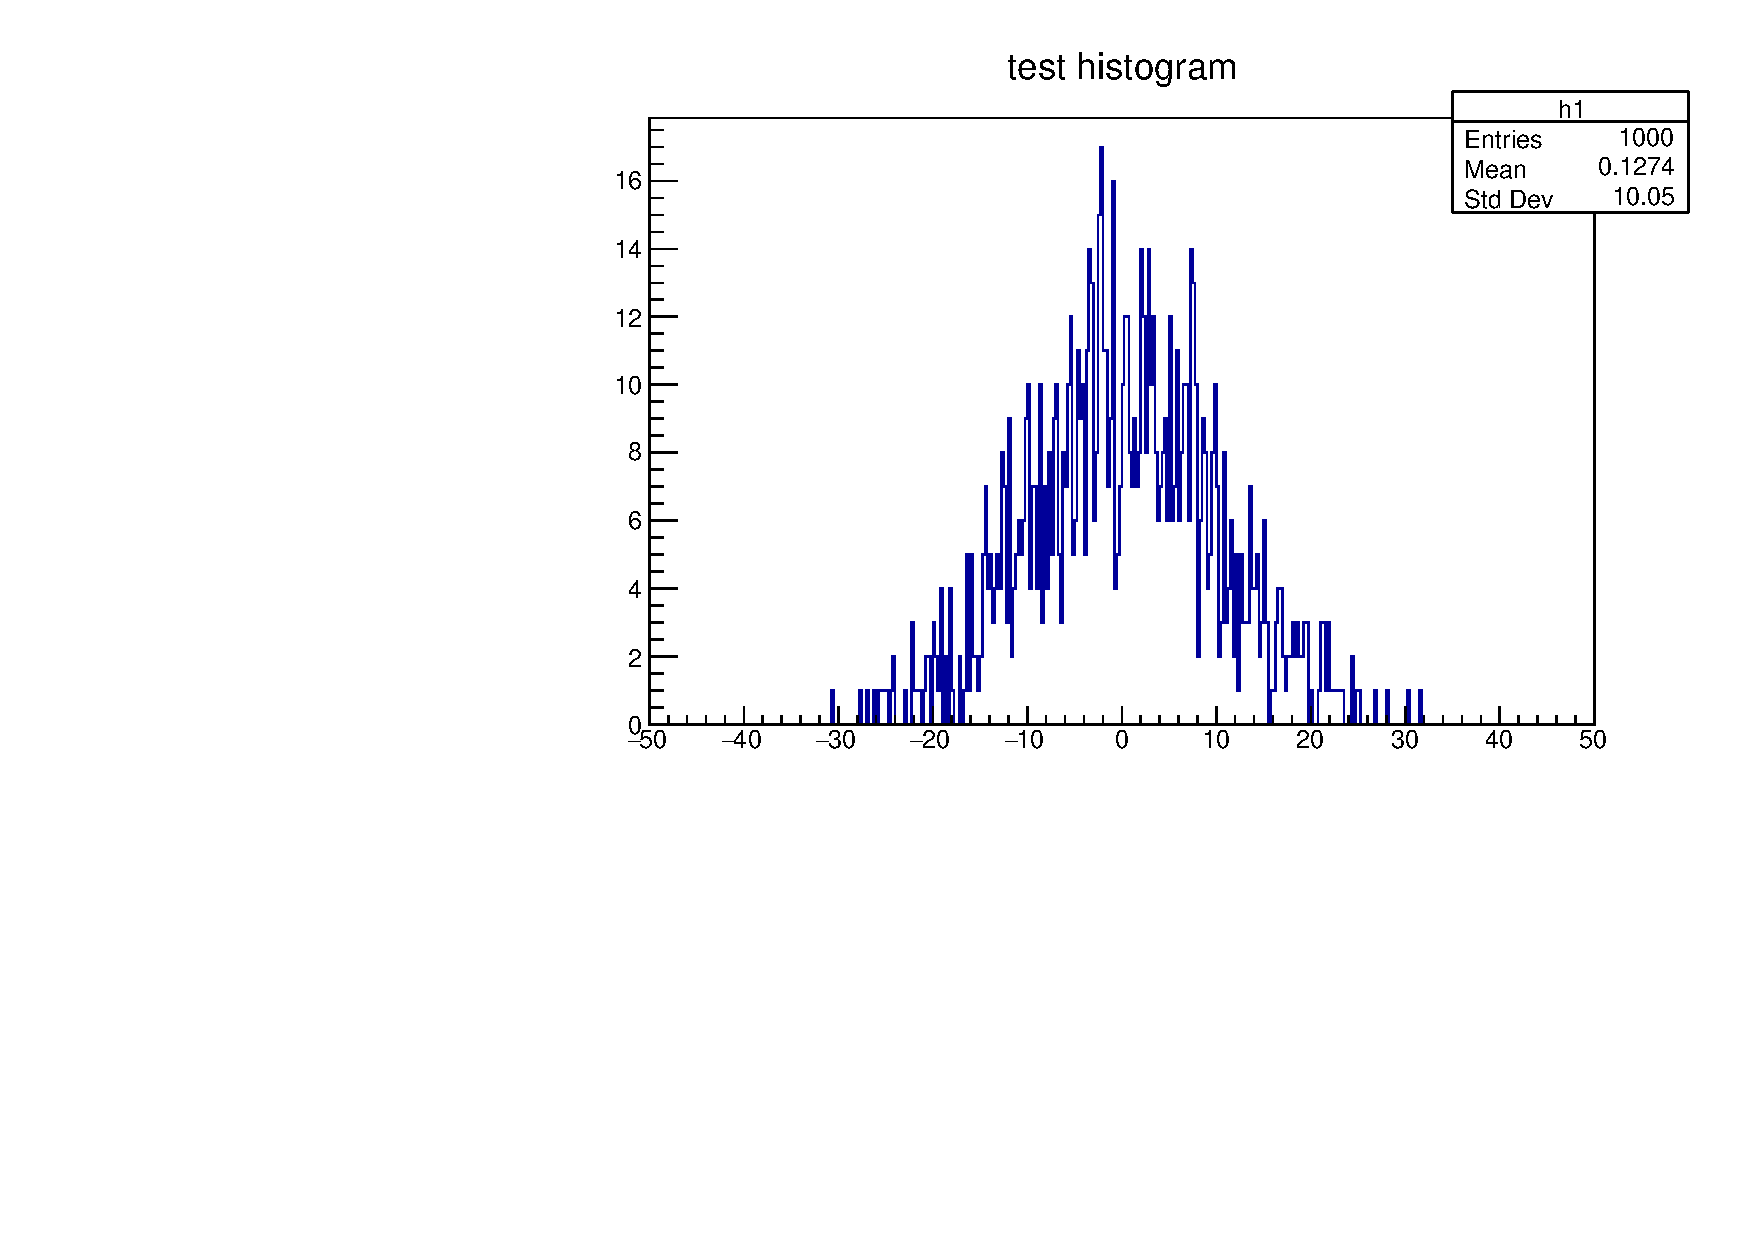
\includegraphics[width=0.6\columnwidth]{testHistogram_01.pdf}
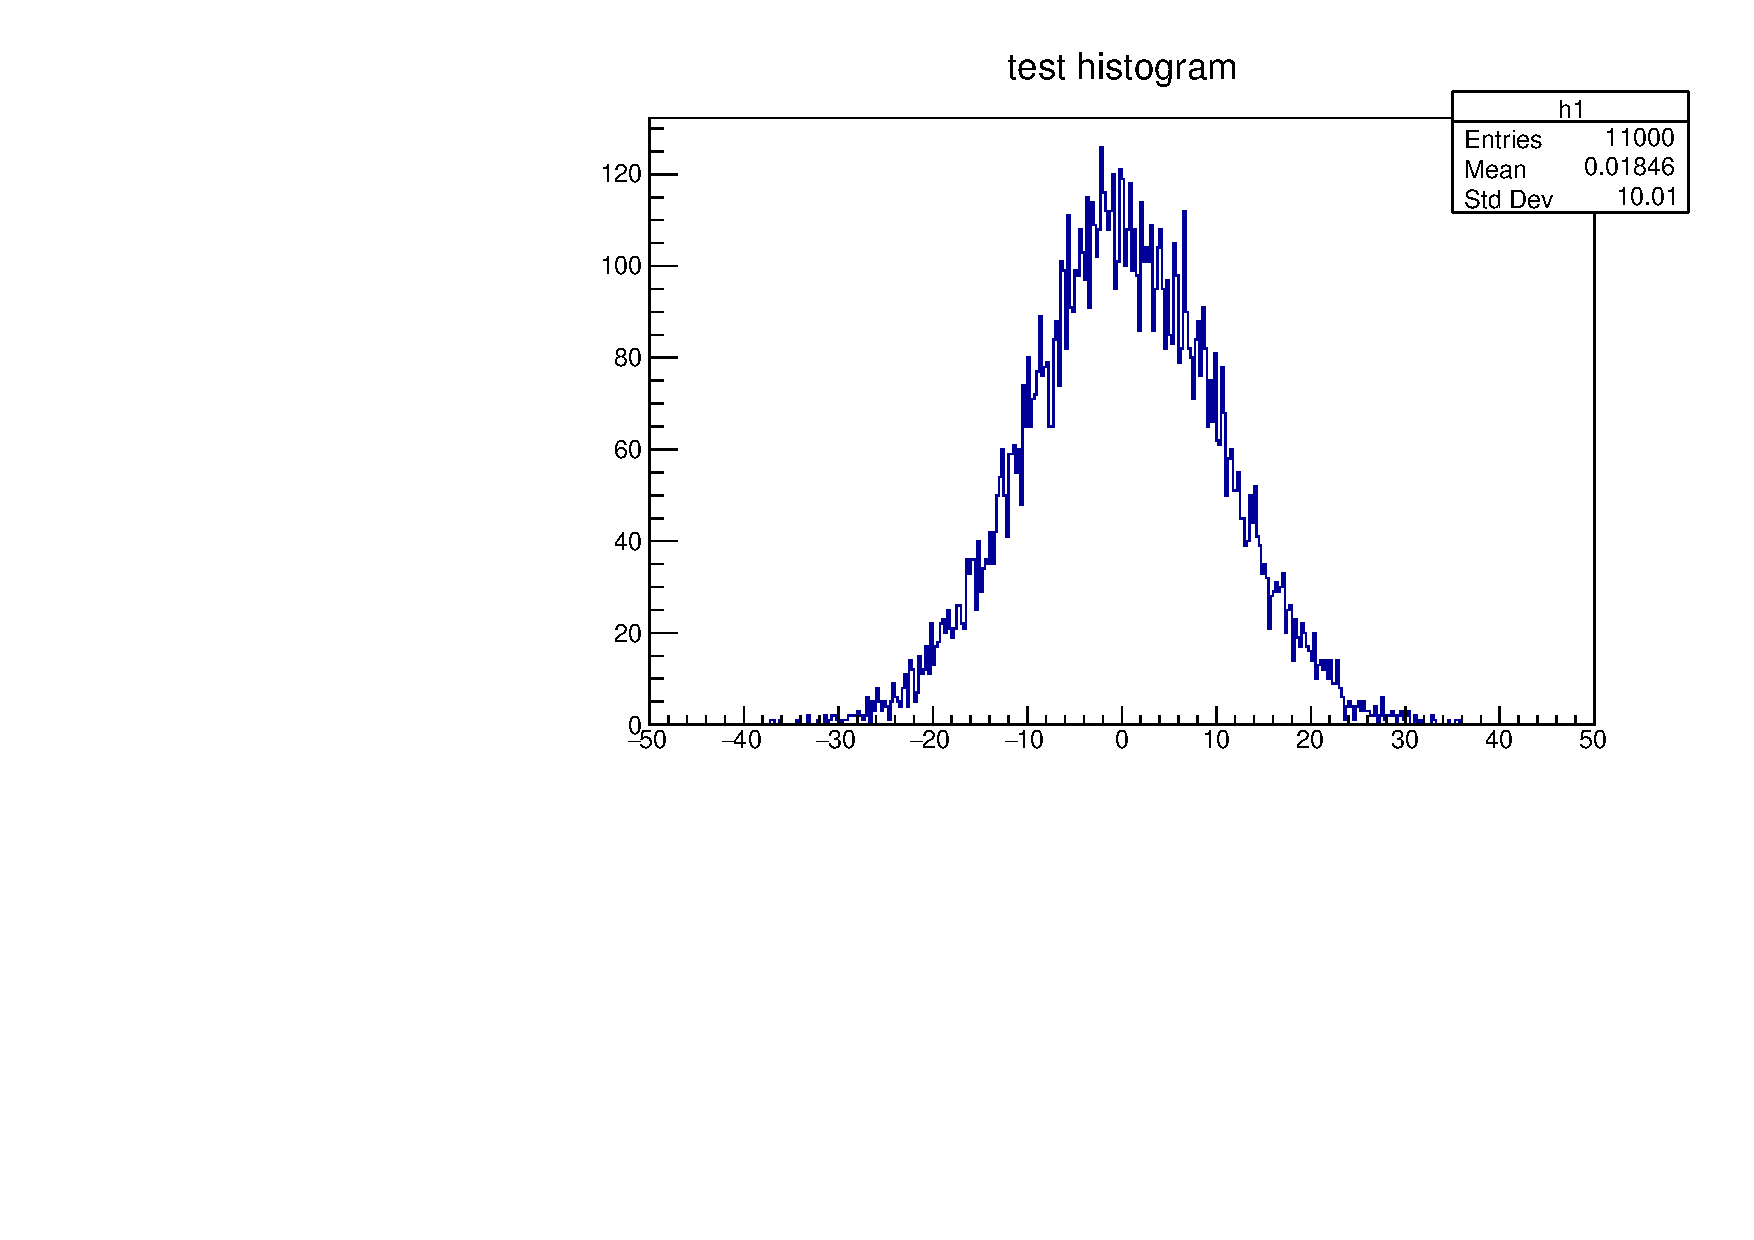
\includegraphics[width=0.6\columnwidth]{testHistogram_02.pdf}
\end{center}
\caption{\label{histo_01} The histogram with a gaussion distribution after running 1000 events (top),
  and after processing 10,000 more events (bottom).
}
\end{figure}

We now add some actual analysis of the event data to the project. The
generated empty project skeleton has a few lines of commented-out code
meant for this tutorial, which we now un-comment to get going.

Use your favorite editor and open \verb|MyTest.cc|.

Un-comment line 13 so it reads \verb|TH1F *h1;|.

Un-comment line 23 so we enable the creation of histogram ``h1''.

Un-comment line 37 so we fill histogram ``h1''.

Save the file and run ``make''.

In the code, we now get the 4th value of packet 1003, the one that
makes a gaussian distribution with a RMS of 10000. Since the API call
\verb|iValue(n)| returns integer values, we use the RMS=10000 value
and divide it by 1000, in order to get a smooth distribution with RMS=10. 

Just as before, we open the test event stream, and run 1000 events. Then we display
histogram ``h1'':

\begin{verbatim}
$ root -l
root [0] #include "MyTest.h"
root [1] .L libMyTest.so
Welcome to pmonitor.  Type phelp() for help
root [2] ptestopen();
root [3] prun(1000);
root [4] h1->Draw();
Info in <TCanvas::MakeDefCanvas>:  created default TCanvas with name c1
root [5]
\end{verbatim}

We get the display shown in Fig.~\ref{histo_01} (top).


After we process 10,000 more events with \verb|prun(10000)|, the
distribution gets smoother, as shown in the lower part of
Fig~\ref{histo_01}.

We have so far used the \verb|prun| command, and were careful to
always specify a number of events (1000 and 10000), so the event loop
actually ends - remember that the test stream has no end. Had we
specified \verb|prun()| or the equivalent \verb|prun(0)|, we would
never have seen the root prompt again. With \verb|prun|, the actions
we specify are executed \emph{synchronously}. So we can issue the next
command only after the \verb|prun| command has ended, even though the
processing of even 10000 events may seem to finish right away. (Later,
convince yourself that this is true by running a much larger number of
events, 500,000 or so.)

\subsection{True Online Monitoring}


We will switch now to actual online monitoring as advertised at the
beginning of this chapter, and will issue \verb|pstart()|. This
command sends the processing of events to the background, and we get
the root prompt back right away.

Issuing \verb|pstart()| here is safe -- since we retain control of the
command prompt, we can always issue \verb|pstop()| to end the
event loop. The subsequent
\verb|pstatus()| commands I issue here show an increasing number of events being
processed in the background:

\begin{verbatim}
root [10] pstart();
root [11] pstatus();
Running at Event 225243  Stream open:   -- testEventiterator (standard)
root [12] pstatus();
Running at Event 317125  Stream open:   -- testEventiterator (standard)
root [13] pstatus();
Running at Event 396368  Stream open:   -- testEventiterator (standard)
root [14] pstop();
\end{verbatim}

\begin{figure}[htb]
\begin{center}
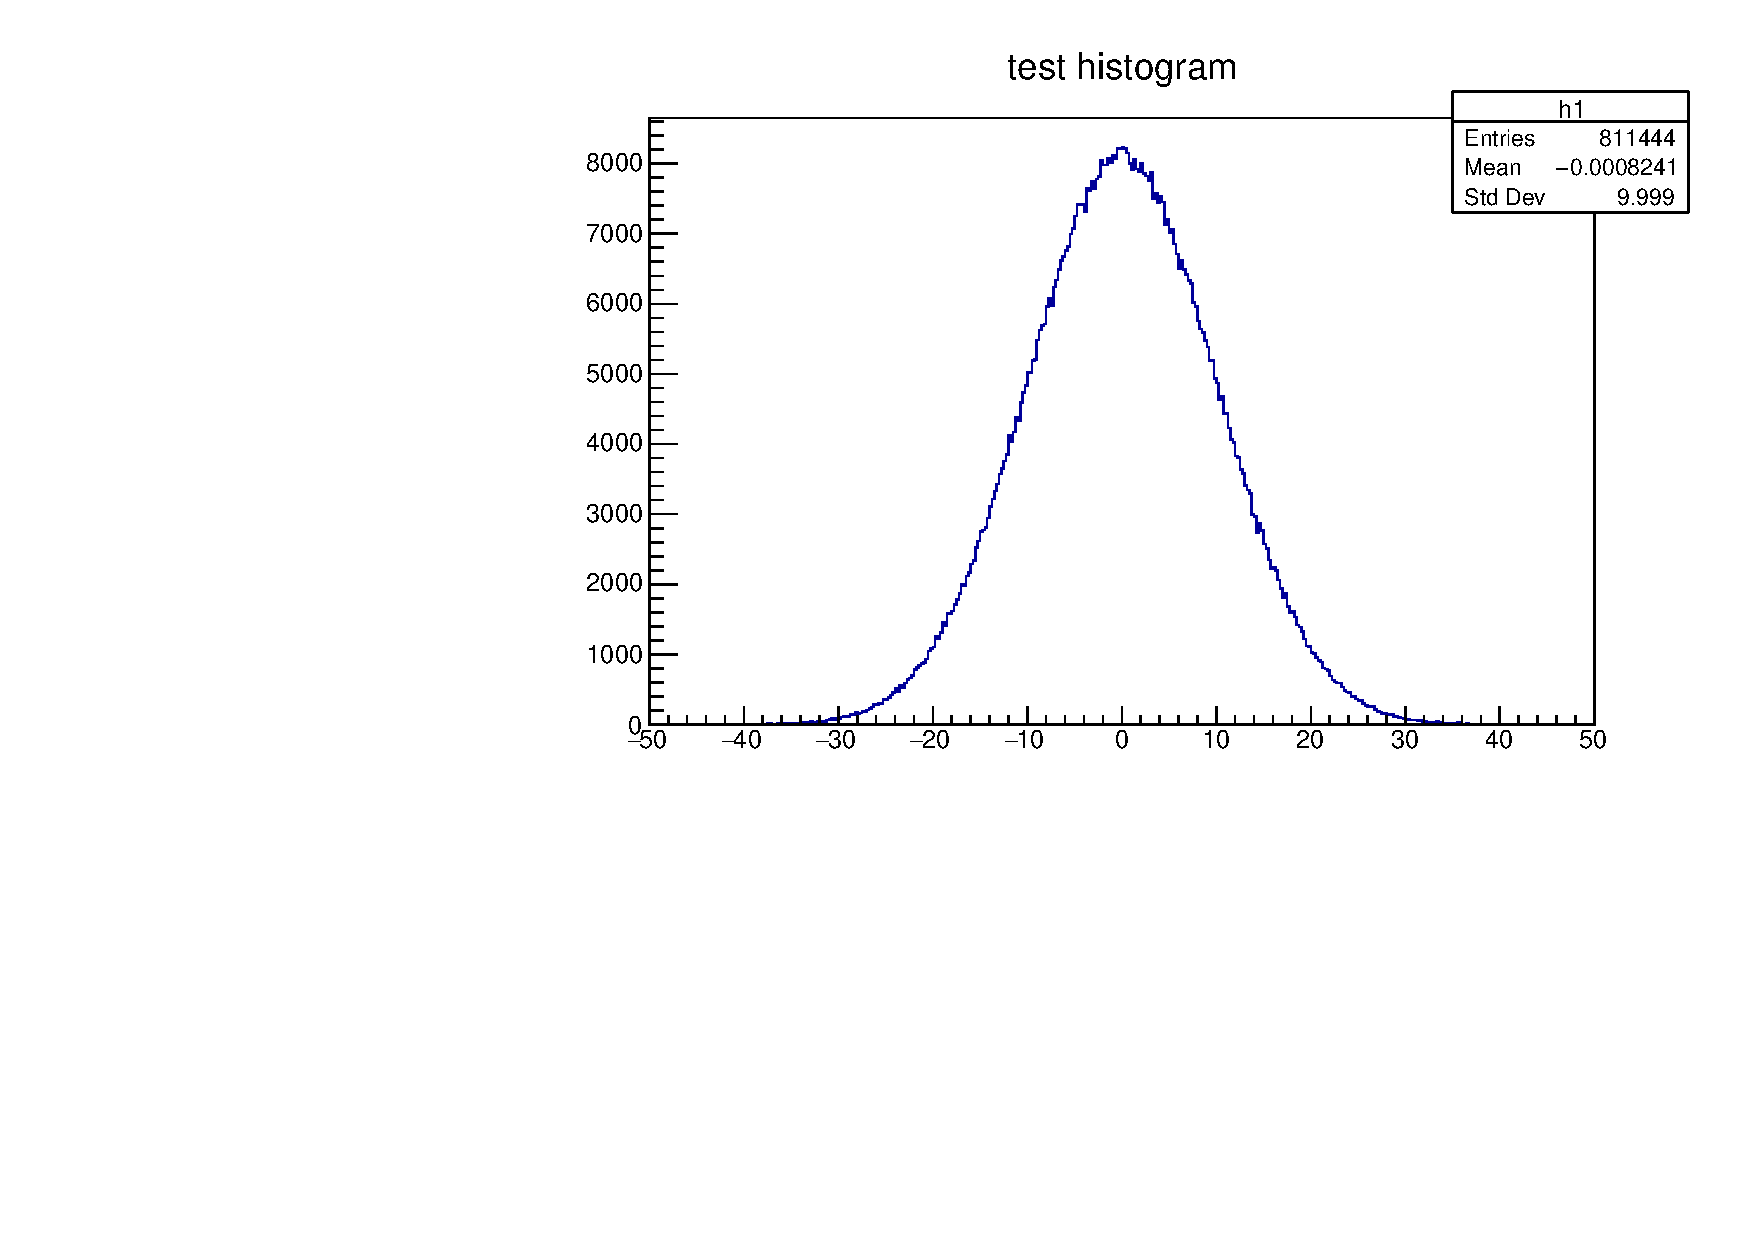
\includegraphics[width=0.6\columnwidth]{testHistogram_03.pdf}
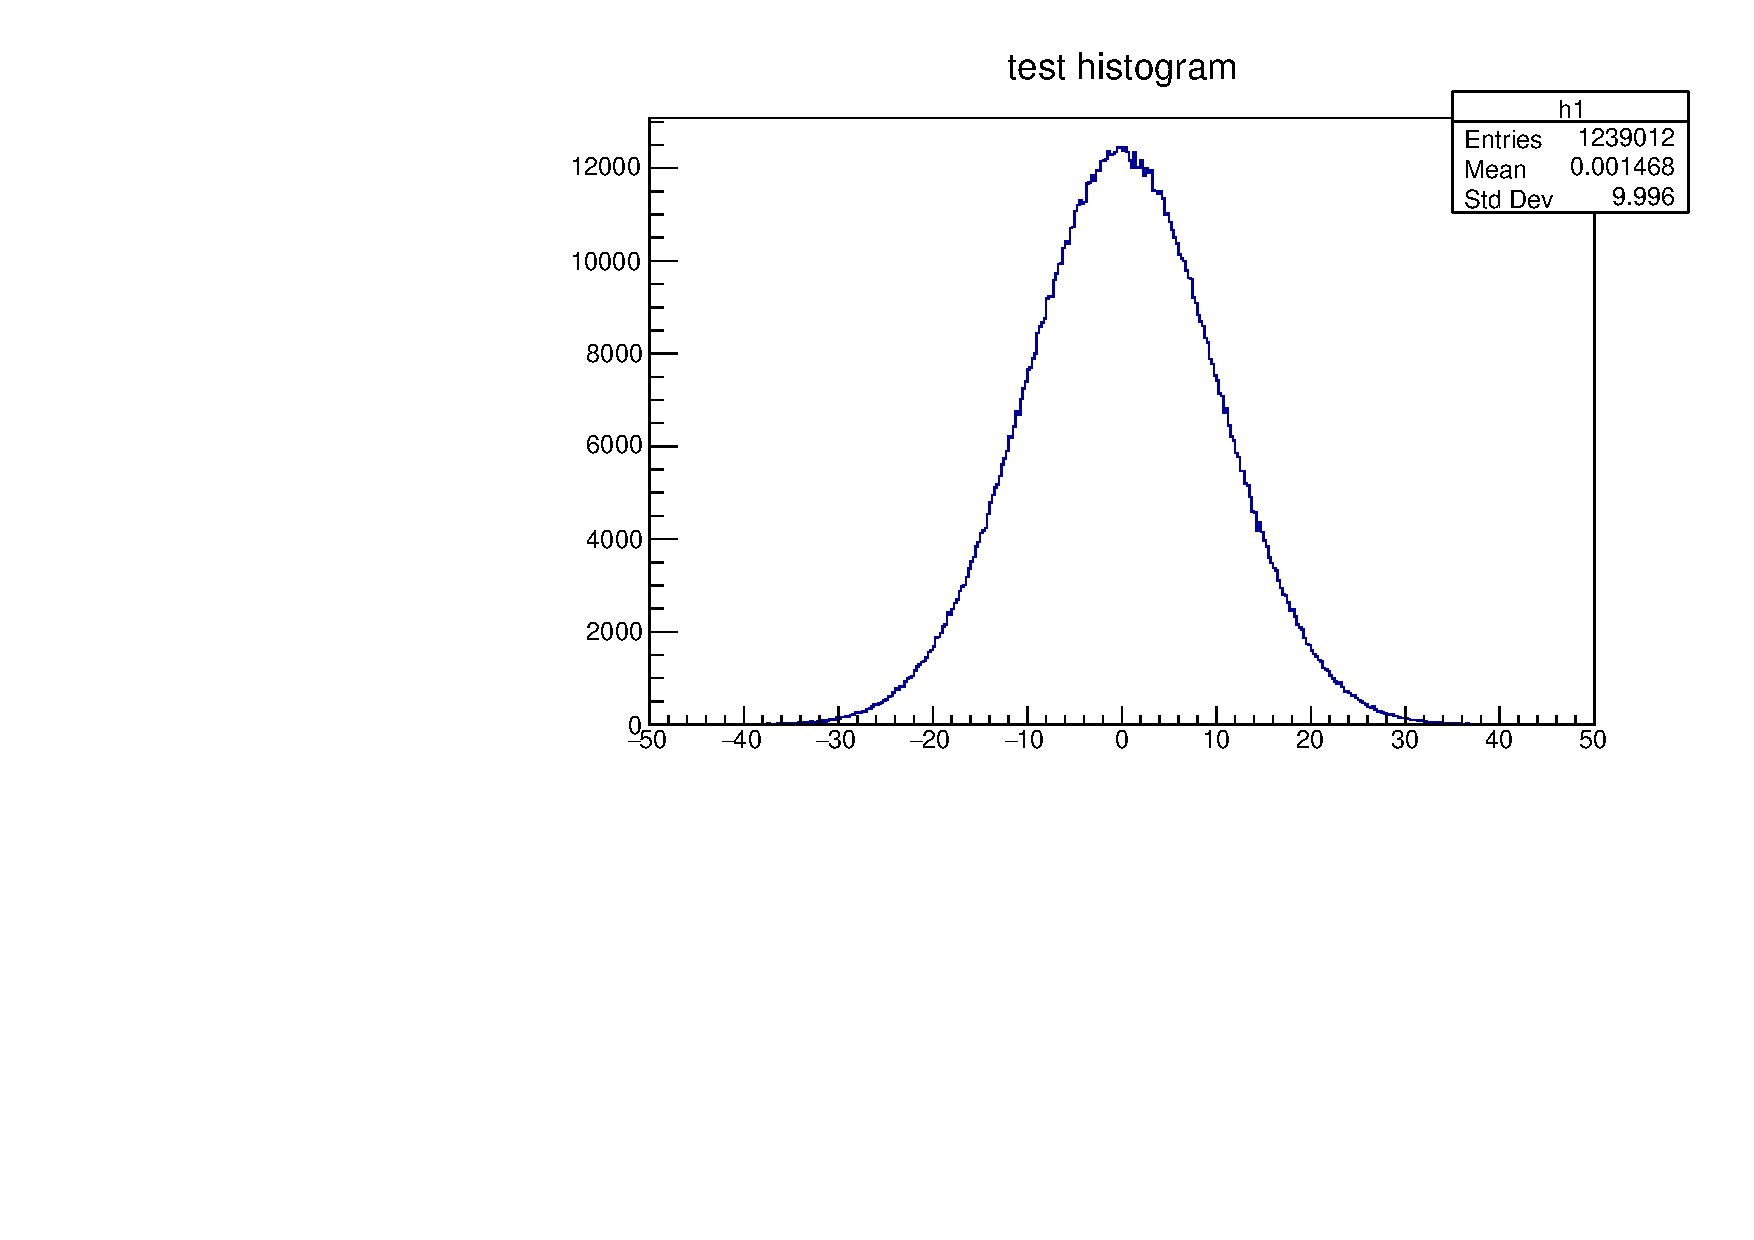
\includegraphics[width=0.6\columnwidth]{testHistogram_04.pdf}
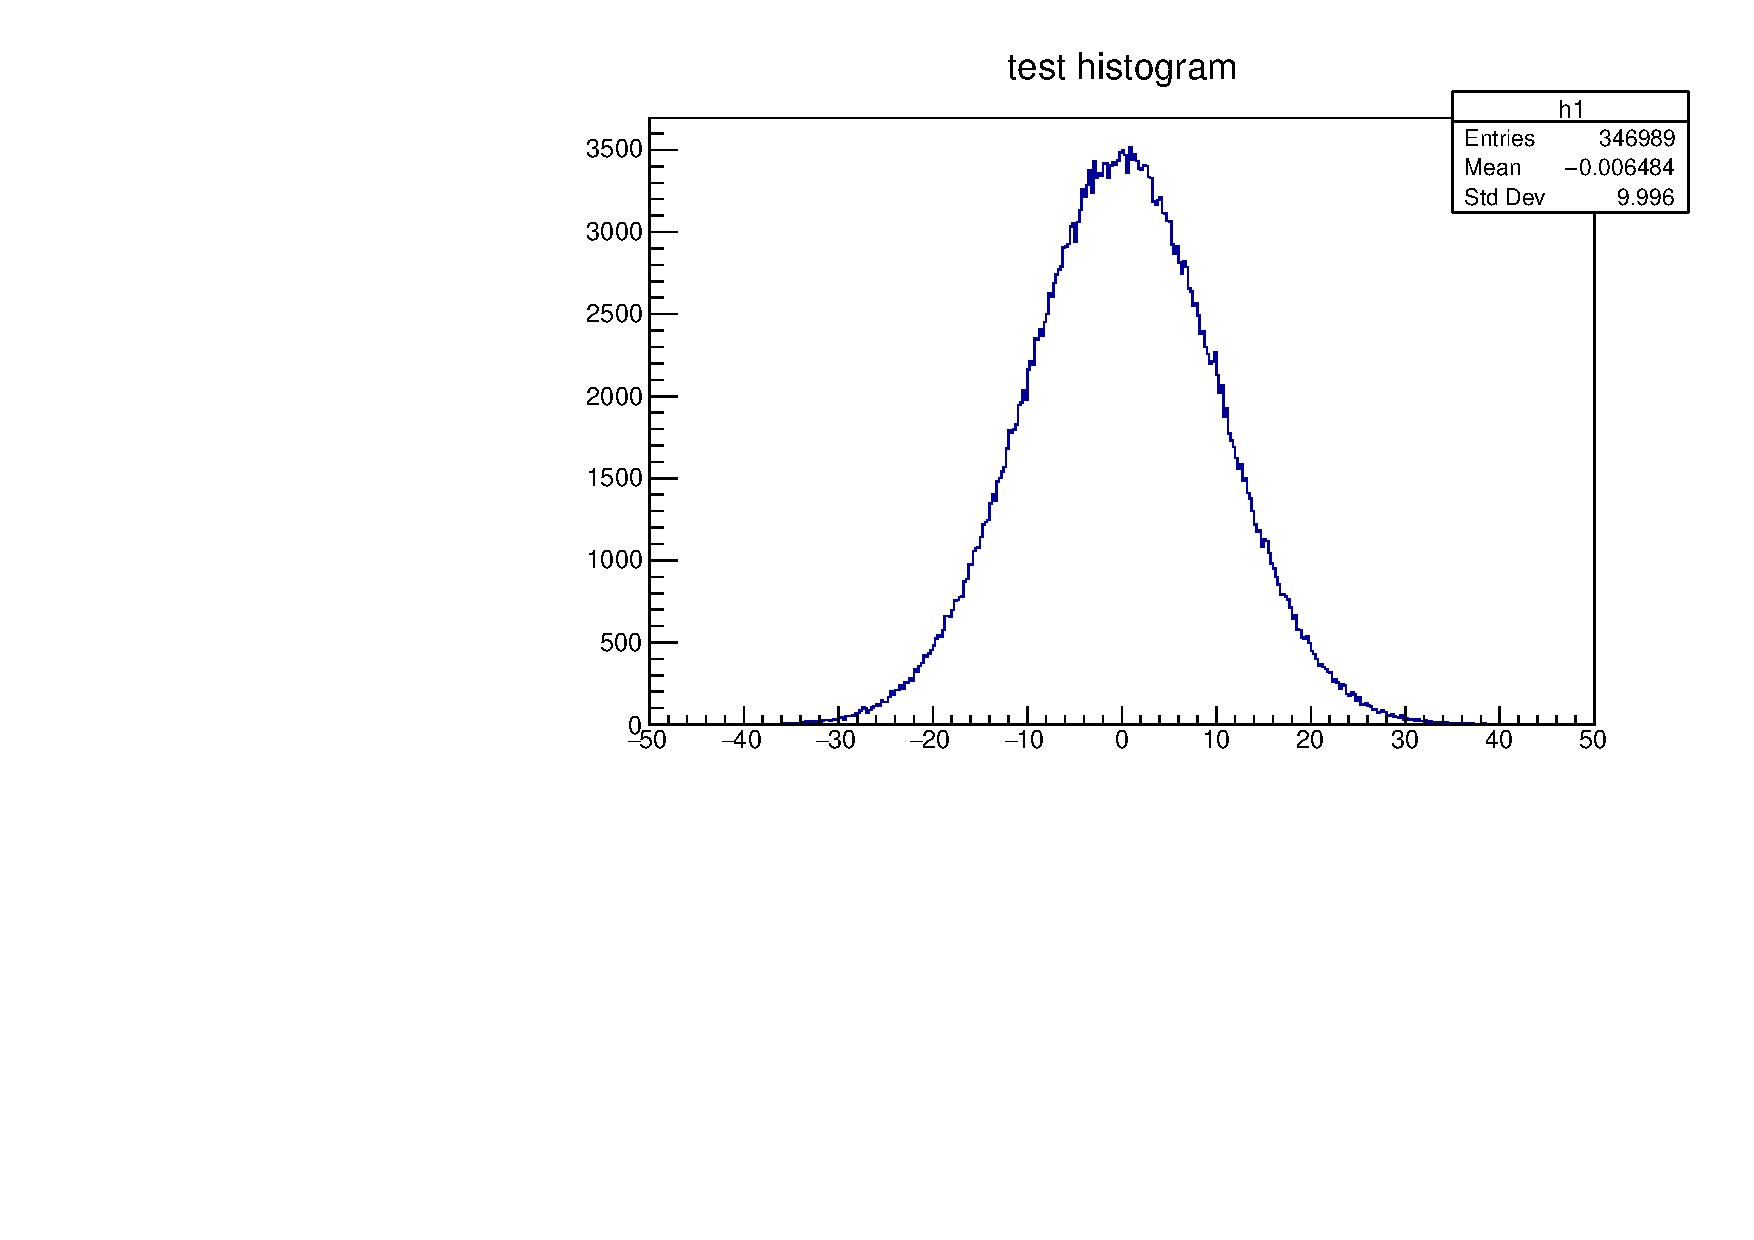
\includegraphics[width=0.6\columnwidth]{testHistogram_05.pdf}
\end{center}
\caption{\label{histo_02} Updating the histogram while it is being filled
  in the background. After the first two updates, I had reset the histogram. 
}
\end{figure}

Each time we click on and so update our histogram display, we see more
entries in the histogram, as shown in Fig~\ref{histo_02}.

This is \emph{true online monitoring}. At any time, we have an active
root prompt and can display or otherwise manipulate the histograms
\emph{while} they are being filled. After clicking and updating twice,
I issued \verb|h1->Reset()|, and the filling of the histogram started
over.

\begin{figure}[htb]
\begin{center}
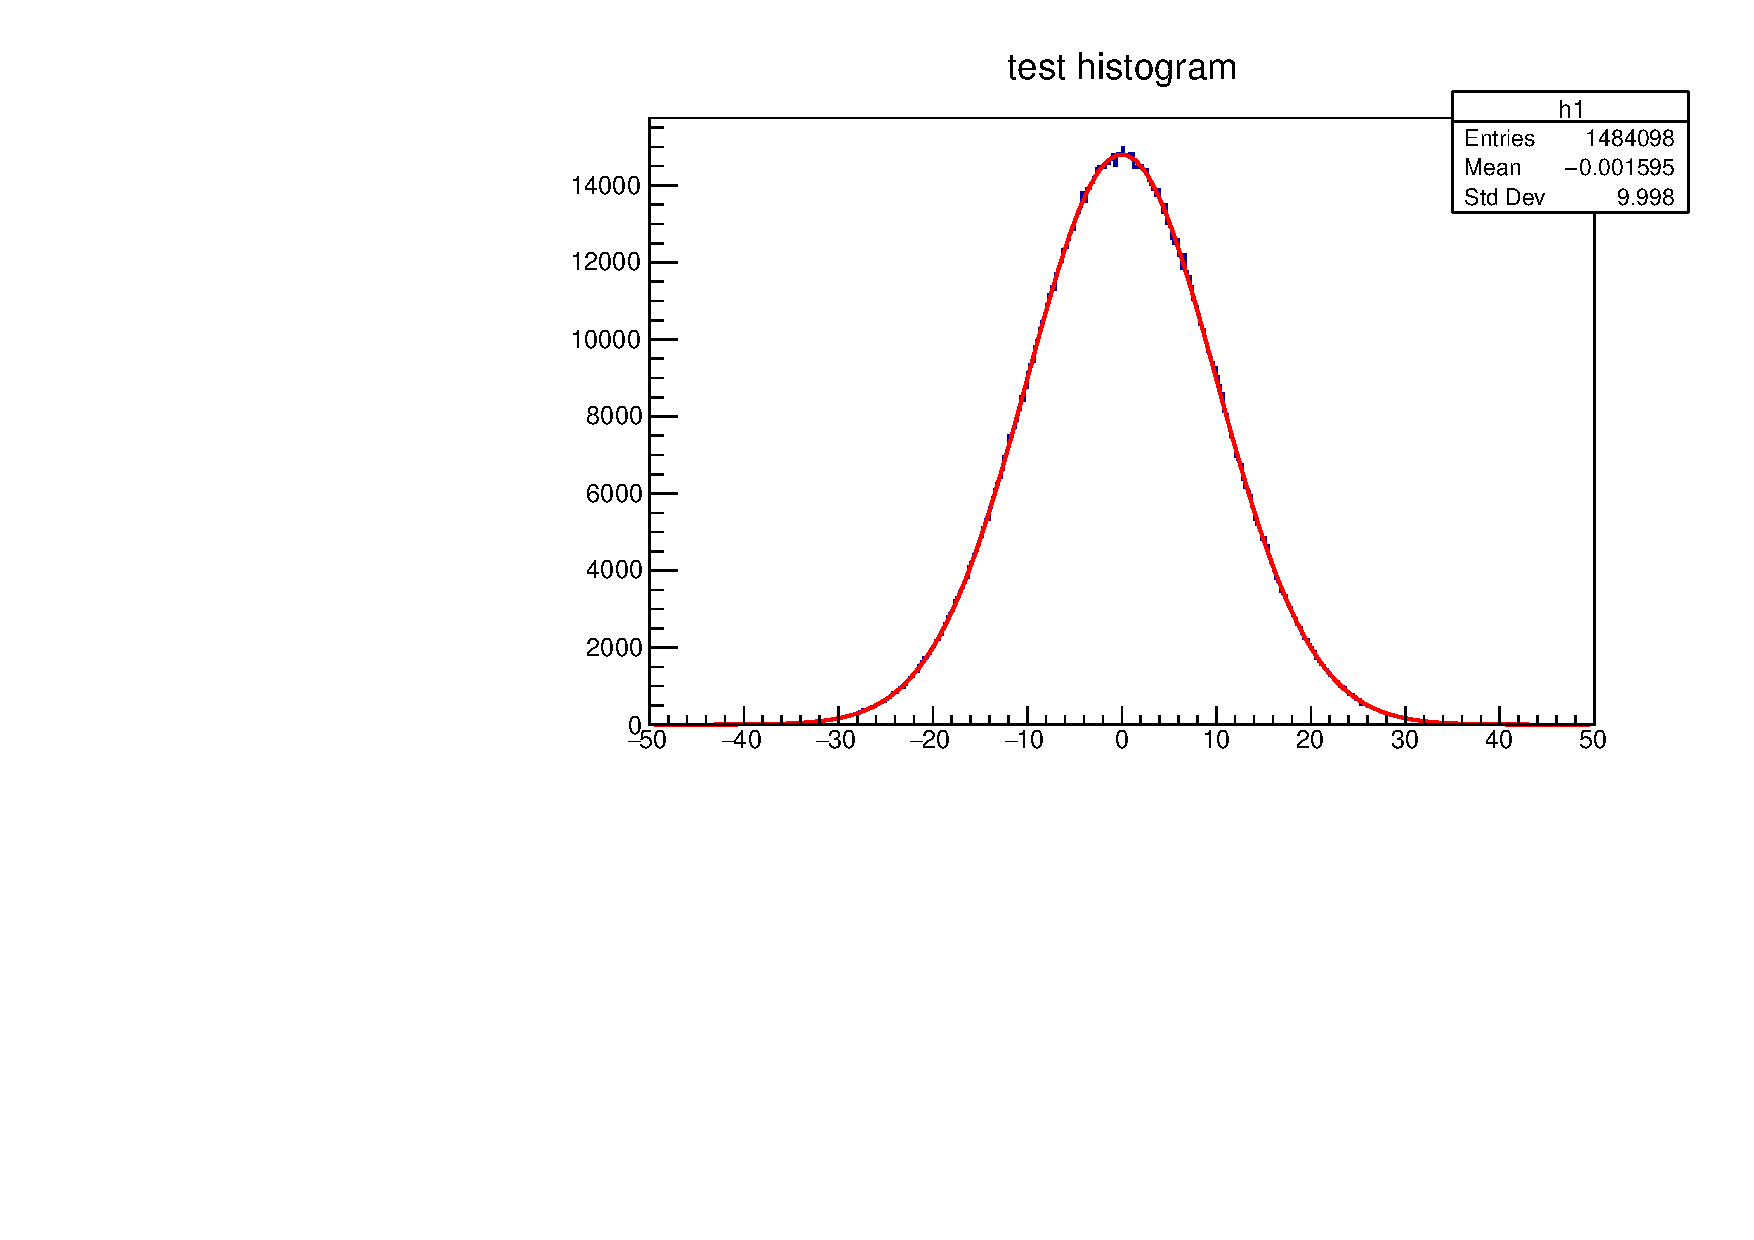
\includegraphics[width=0.6\columnwidth]{testHistogram_06.pdf}
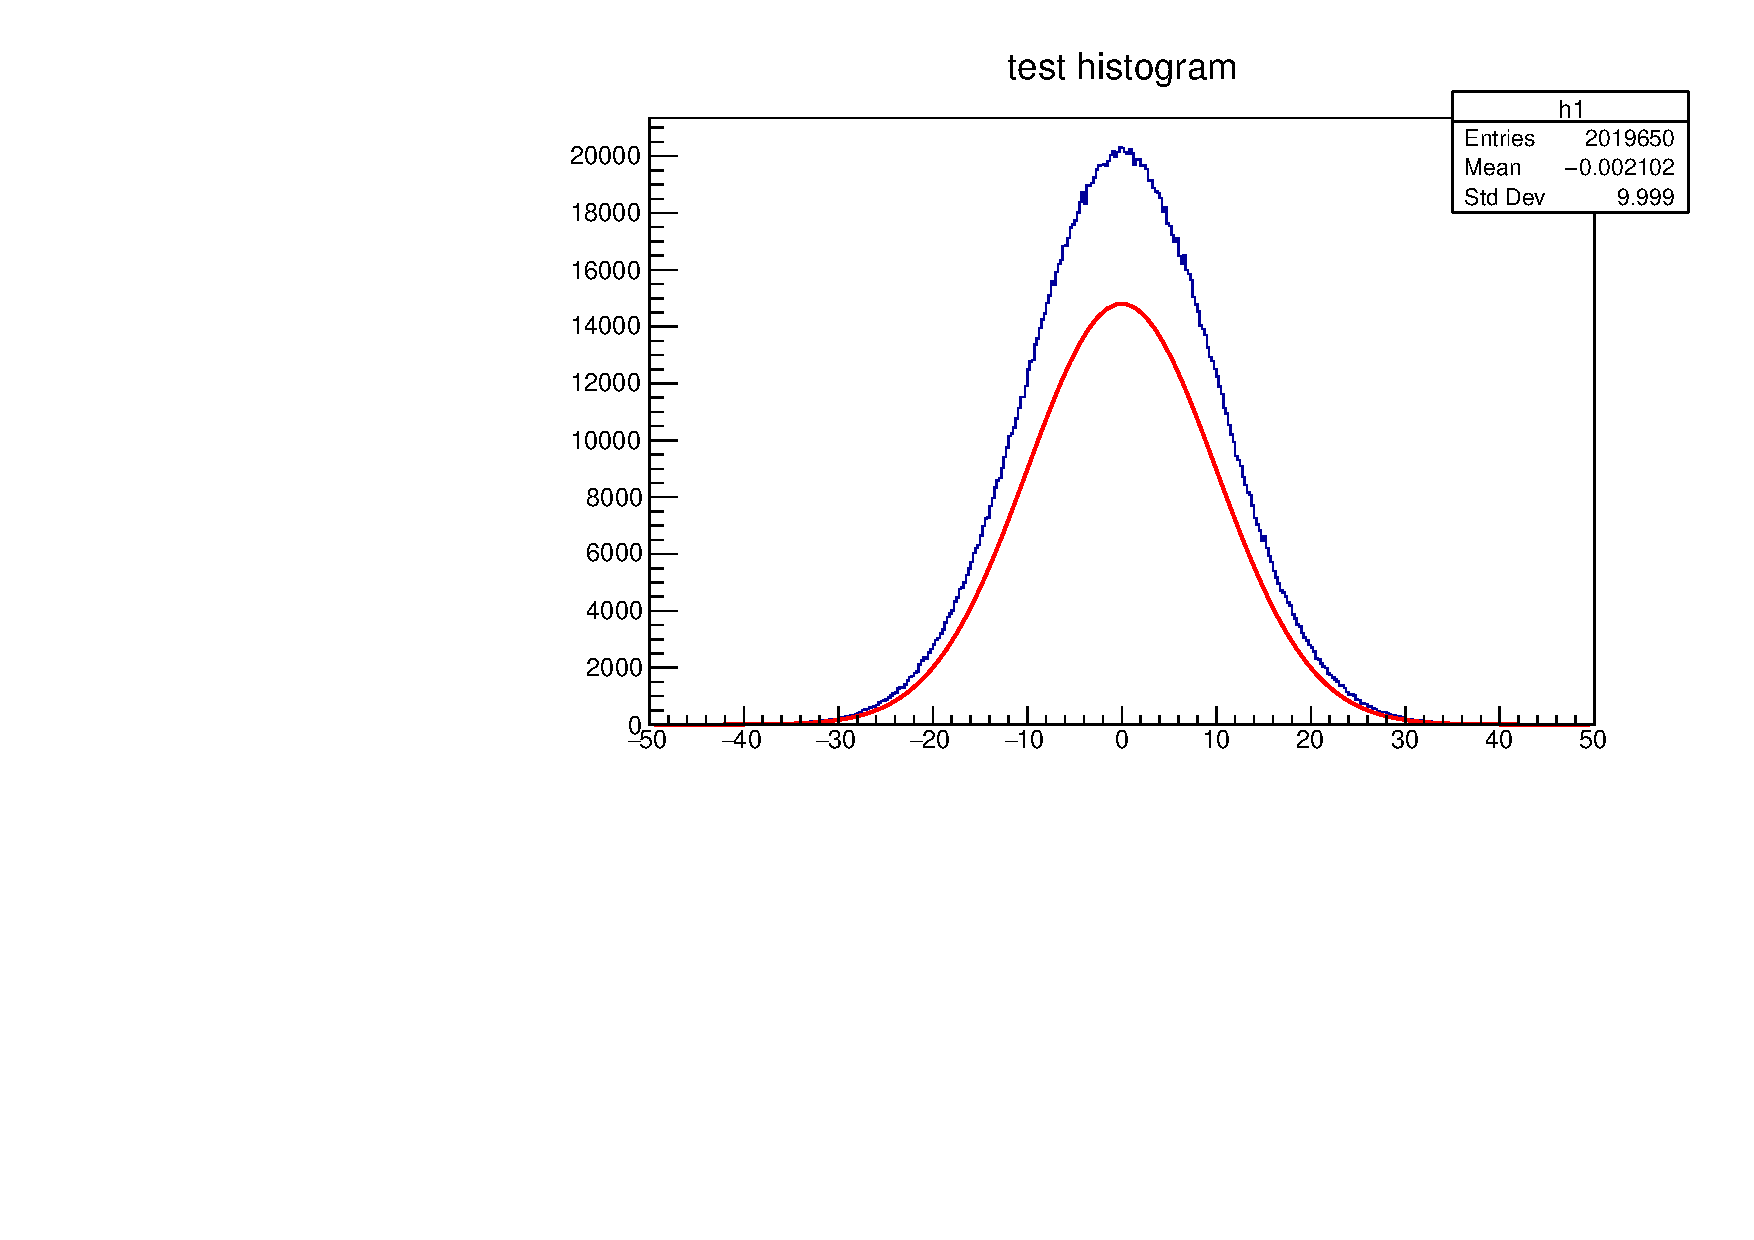
\includegraphics[width=0.6\columnwidth]{testHistogram_07.pdf}
\end{center}
\caption{\label{histo_fit} The effect of fitting a gaussian curve to
  the histogram as it is being filled. The fitted curve fits the
  distribution nicely (top).  But since we continue to update the histogram,
  the fit curve is ``left behind'' when we update next (bottom). 
}
\end{figure}


This gets even more tangible when we fit a gaussian to the histogram:

\begin{verbatim}
root [21] h1->Fit("gaus");
 FCN=371.775 FROM MIGRAD    STATUS=CONVERGED      55 CALLS          56 TOTAL
                     EDM=1.91072e-07    STRATEGY= 1      ERROR MATRIX ACCURATE
  EXT PARAMETER                                   STEP         FIRST
  NO.   NAME      VALUE            ERROR          SIZE      DERIVATIVE
   1  Constant     1.48104e+04   1.48711e+01   1.14626e-01  -6.31547e-06
   2  Mean        -1.05490e-03   8.20375e-03   7.73406e-05   7.46670e-02
   3  Sigma        9.99178e+00   5.77768e-03   1.48519e-06  -4.36377e-01
root [22]
\end{verbatim}

At first, the fit describes the distribution nicely. But as we update
again, since the background processing keeps updating the histogram, the
fit is ``left behind'' (Fig~\ref{histo_fit}).


\subsection{Online Monitoring an Online Stream}

I have set up the example so the exact same code can be run directly
from the RCDAQ data acquisition. RCDAQ comes with a pseudo device that
makes packets exactly like the test stream's packet 1003, except that
they are now generated by the data acquisition, and you can get them
by opening an online stream that requests data from RDCAQ directly.

The RCDAQ discribution comes with a setup script \verb|setup_pmonitor_tutorial.sh|
that sets RCDAQ up just for this purpose.

Execute that script, and start a run (by \verb|daq_begin| or a GUI).
(No need to open a data file!)


In the monitoring process,
\begin{itemize}
\item issue \verb|rcdaqopen()|
\item issue \verb|pstart()|
\item for good measure, issue \verb|pstatus()|
\item dislay the histograms as shown in the previous chapter
\end{itemize}



\subsection{Billboard-Style Displays}

So far I have shown that the histogram updates each time I click on
the display. Very often, I find myself using this really interactive
online monitoring. However, often one wants ``billboard-style''
displays that are possibly displayed on an overhead monitor and that
update periodically.

There are two ways to accomplish this. The first (and easiest) way is
to schedule periodic updates, for example, update a particular canvas
every 30 seconds. Different canvases can have individual refresh
times. This is easiest because you can use this method for canvases that
you dynamically create, including those that are created implicitly,
for example, when you execute a ``Draw()'' function, as in
\begin{verbatim}
h1->Draw();
\end{verbatim}
The downside of this method is that the updates happen asynchronously
on a timer, and are not correlated to anything else going on. Also,
the updates continue even though no events might get processed
at that moment.

The other method is to schedule updates at times determined by your
program, most often in your \verb|process_event| routine. In order for
that to work, you need to explicitly create a Root \verb|TCanvas| in
your code so the pointer to it is accessible from your code.

\verb|pmonitor| provides a user-callable function
\begin{verbatim}
updatePad( TVirtualPad *);
\end{verbatim}
that you can call at any time to update the canvas.

For example, you could call this method in your \verb|process_event|
function on receipt of special events such as the begin-run or end-run
events. Let's say that \verb|canvas_a| is a pointer to a TCanvas object:

\begin{verbatim}
  if ( e->getEvtType() == ENDRUNEVENT )
    {
      if (canvas_a) updatePad(canvas_a);
    }
\end{verbatim}

In addition, you could update the canvas every 500 events:

\begin{verbatim}
  if ( (e->getEvtSequence() % 500) == 0)
    {
      if (canvas_a) updatePad(canvas_a);
    }
\end{verbatim}

The advantage is that you see the final histograms after a run ends,
and see updates every 500 events, but do not update when you are not
processing events. You could also decide to update after an
``interesting'' event has been found.

Once you have made a root ``TCanvas'' display (that can have divisions
and sub-panels), you can request an automatic, periodic update by

\begin{verbatim}
pupdate(c1, 30);
\end{verbatim}

\verb|c1| is the pointer to the TCanvas that you either explicitly
created, or, as in the examples before, was implicitly created by
issuing \verb|h1->Draw()|. The above command makes the Canvas update
itself every 30 seconds. If you have multiple TCanvas displays, you can
specify individual update frequencies for each display:

\begin{verbatim}
pupdate(c1, 15);
pupdate(c2, 30);
\end{verbatim}

It is only neccessary to give the top-level TCanvas pointer as the
argument; the update routine updates all sub-structures on the Canvas,
if any. Let me also point out that you can give a sub-pad as the
argument to either method (they take a pointer to a
\verb|TVirtualPad *| as their argument), and update portions of a
canvas, or, for more complex ones, update portions at different
times or intervals.

\pointout{For complex displays with sub-pads and especially
  ``Lego''-style plots, make sure that you do not request too short an
  update interval. The re-drawing of complex graphics takes time, and
  slows down the processing. For complex graphics, you should not go
  below a 30s interval.
}

In order to end the automatic update for a given Canvas \verb|c1|, issue

\begin{verbatim}
pendupdate(c1);
\end{verbatim}

Issuing

\begin{verbatim}
pendupdate();
\end{verbatim}

will end the updates for \emph{all} Canvases that were updating.

%\appendix

%Section 



\end{document}


